\documentclass[journal]{IEEEtran}
%\usepackage{wrapfig}
% \usepackage{amsmath}
 \usepackage{url,cite}
\usepackage{rotating}
\usepackage{color, colortbl}
\usepackage{graphicx}

%\usepackage{program}
\usepackage{cite}
\usepackage{alltt}
\newcommand{\eq}[1]{Equation~\ref{eq:#1}}
\newcommand{\bi}{\begin{itemize}}
\newcommand{\ei}{\end{itemize}}
\newcommand{\be}{\begin{enumerate}}
\newcommand{\ee}{\end{enumerate}}
\newcommand{\tion}[1]{\textsection\ref{sec:#1}}
\newcommand{\fig}[1]{Figure~\ref{fig:#1}}
\definecolor{lightgray}{gray}{0.975}
\usepackage{fancyvrb}
\usepackage{stfloats}
\usepackage{multirow}
\usepackage{listings}
\usepackage{subcaption}
\usepackage{algorithmicx}

\usepackage{enumitem}
\setitemize{noitemsep,topsep=0pt,parsep=0pt,partopsep=0pt}



\newcommand{\ADD}[1]{#1}

\definecolor{MyDarkBlue}{rgb}{0,0.08,0.45} 
\newenvironment{changed}{\par}{\par}


\definecolor{darkgreen}{rgb}{0,0.3,0}

\usepackage[table]{xcolor}
\definecolor{Gray}{rgb}{0.88,1,1}
\definecolor{Gray}{gray}{0.85}
\definecolor{Blue}{RGB}{0,29,193}
 
 
%\newcommand{\JOE}[1]{\textcolor{red}{\bf{ JOE: #1 !!!}}}
\newcommand{\RED}[1]{\textcolor{red}{\bf{ JOE: #1 !!!}}}
%\newcommand{\TIM}[1]{\textcolor{Blue}{\bf{ TIMM: #1 !!!}}}
\newcommand{\G}{\cellcolor{green}}
\newcommand{\Y}{\cellcolor{yellow}}

\usepackage{todo}

\begin{document}

%Learning Effective Pilot Operation Strategies with a Cognitive Model for Safe Aircraft Approach
\title{Better Model-Based Analysis of\\ Human Factors for Safe Aircraft Approach}


\author{Joseph~Krall\thanks{Joseph Krall  
is a postdoctoral research fellow at LoadIQ, Reno, Nevada;
e-mail: kralljoe@gmail.com}, %
Tim~Menzies~\IEEEmembership{Member,~IEEE}\thanks{Tim Menzies is with the Computer Science department, NcState University; email:  tim.menzies@gmail.com.}, %
Misty Davies~\IEEEmembership{Member,~IEEE}
\thanks{
Misty Davies is with the Intelligent Systems Division,
NASA Ames Research Center, CA, USA;
e-mail:
misty.d.davies@nasa.gov.}
}

\maketitle
%\IEEEcompsoctitleabstractindextext{%
\begin{abstract}
%Modern model-based methods can assess if the requirements for cockpit operation
%can exceed the 
%cognitive capacity of human pilots. For example,
%this paper explores
%the Work Models that Compute (WMC) framework for human behavior of pilots (working together with automated controls) in the cockpit of an aircraft during an airplane's approach to the runway.  

%For example,
%in this paper we   use WMC to  describe limitations to the size of a task load that a pilot can handle before flight operations become unsafe (due to average delays in completing the task load). We also show that  such limitations only exist due to the overly complex nature of flying aircraft  \TIM{to wimpy?}.
%\JOE{Misty says: Joe, I'm not sure I agree with the final statement in the abstract. Can you tell me what you were trying to say in a different way? }

How can analysts better reason about the complex interactions between humans and machines in safety critical systems? 
For example, consider the complexities arising when
a large commercial aircraft makes a runway approach.
At that time, pairs of pilots interact with both each other and a
large number of intricate on-board automated systems.  
Any model of that kind of pilot interaction is inherently complex and, therefore, inherently hard to commission, debug, and study.

We advocate exploring complex models by combining data miners (to find a small set of most critical examples) and of multi-objective optimizers (that focus on  those critical examples). 
An example of such a combination is the GALE optimizer that intelligently explores thousands of scenarios by examining just a few dozen of the most informative examples.  
GALE-style reasoning enables a very fast, very wide-ranging exploration of behaviors, as well as the effects of those behaviors' limitations.




\end{abstract}

\begin{keywords}
Human Factors, Cognitive Modeling, Multi-objective Optimization, Active Learning
\end{keywords}
%}

%\maketitle

\markboth{Name of Journal here,~Vol.~X, No.~Y, January~2014}%
{Shell \MakeLowercase{\textit{et al.}}: Understanding the Impact of Human Factors in a Cognitive Model for Safe Aircraft Approach}


\IEEEdisplaynotcompsoctitleabstractindextext
\IEEEpeerreviewmaketitle



\section{Introduction}
There are many advantages of a model-based approach to human factors. 
Traditional human-in-the-loop experimental case-studies are expensive, time consuming, and difficult to reproduce.
Model-based conclusions, on the other hand, are reproducible and verifiable (just run the model again).
Another advantage of the model-based approach is that models can simulate real world behavior much faster than real-time;
thereby enabling an extensive evaluation of more options than slow-time real-world case studies.

In theory, complex models can be analyzed via multi-objective optimizers by running them across many CPUs. 
In practice, that CPU may not be available.
For example one of us (Davies) regularly analyzes a model that needs 30 weeks of CPU time. 
For high priority issues in need of urgent resolution, then this 30 weeks of computer time can be achieved in five days of parallel execution on NASA's supercomputers.
However,  researchers can usually access a small fraction of that CPU. 
For example, if there has been some incident on a manned space mission,  NASA enlists all available CPU time for ``damage modeling'' (which is a large series of ``what-if'' queries to assess potential impacts). 
At those times, researchers can access zero CPU for any other purpose. 


To address this problem in other domains, we have proposed a new optimization method, called GALE~\cite{krall14aaai,krallphd,galepaper},
that  focuses on a small number of most informative examples.
Hence, GALE explores only a few dozen examples rather than the thousands (or more) used  by traditional methods~\cite{galepaper,krall14aaai}. 
This simplifies and improves our ability to reason about complex cognitive models.

In practice, GALE runs much faster than traditional optimizers. 
Standard optimization algorithms such as NSGA-II~\cite{deb00afast} require 3000 to 5000 evaluations to explore the pilot simulator that is the large study of this paper. 
GALE, on the other hand, performs the same task using 25 to 50 evaluations~\cite{krallphd}.
In practice, this has tremendous practical implications.
When generating conclusions from a randomizing optimizer such as GALE or NSGA-II, it is important to check that the conclusions hold in multiple repeats (say, 20 repeats). 
This number of evaluations is a critical indicator of runtime in optimizers when the model is complex.
For example, a study of the pilot simulator (replicated 20 times)
takes 1.5 and 100 hours for GALE and NSGA-II, respectively~\cite{krallphd}.



\begin{figure*}[!t]
\begin{minipage}{2in}
\noindent
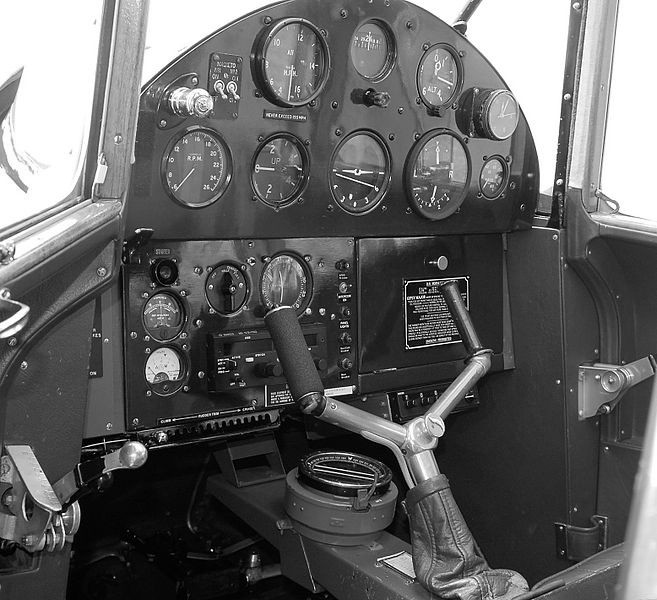
\includegraphics[width=1.6in]{images/HavilandMoth1936GS}

\noindent
Fig.~\ref{fig:sfig}a: Haviland Moth,1936\cite{deHavilandPhoto}.

~\\


\noindent 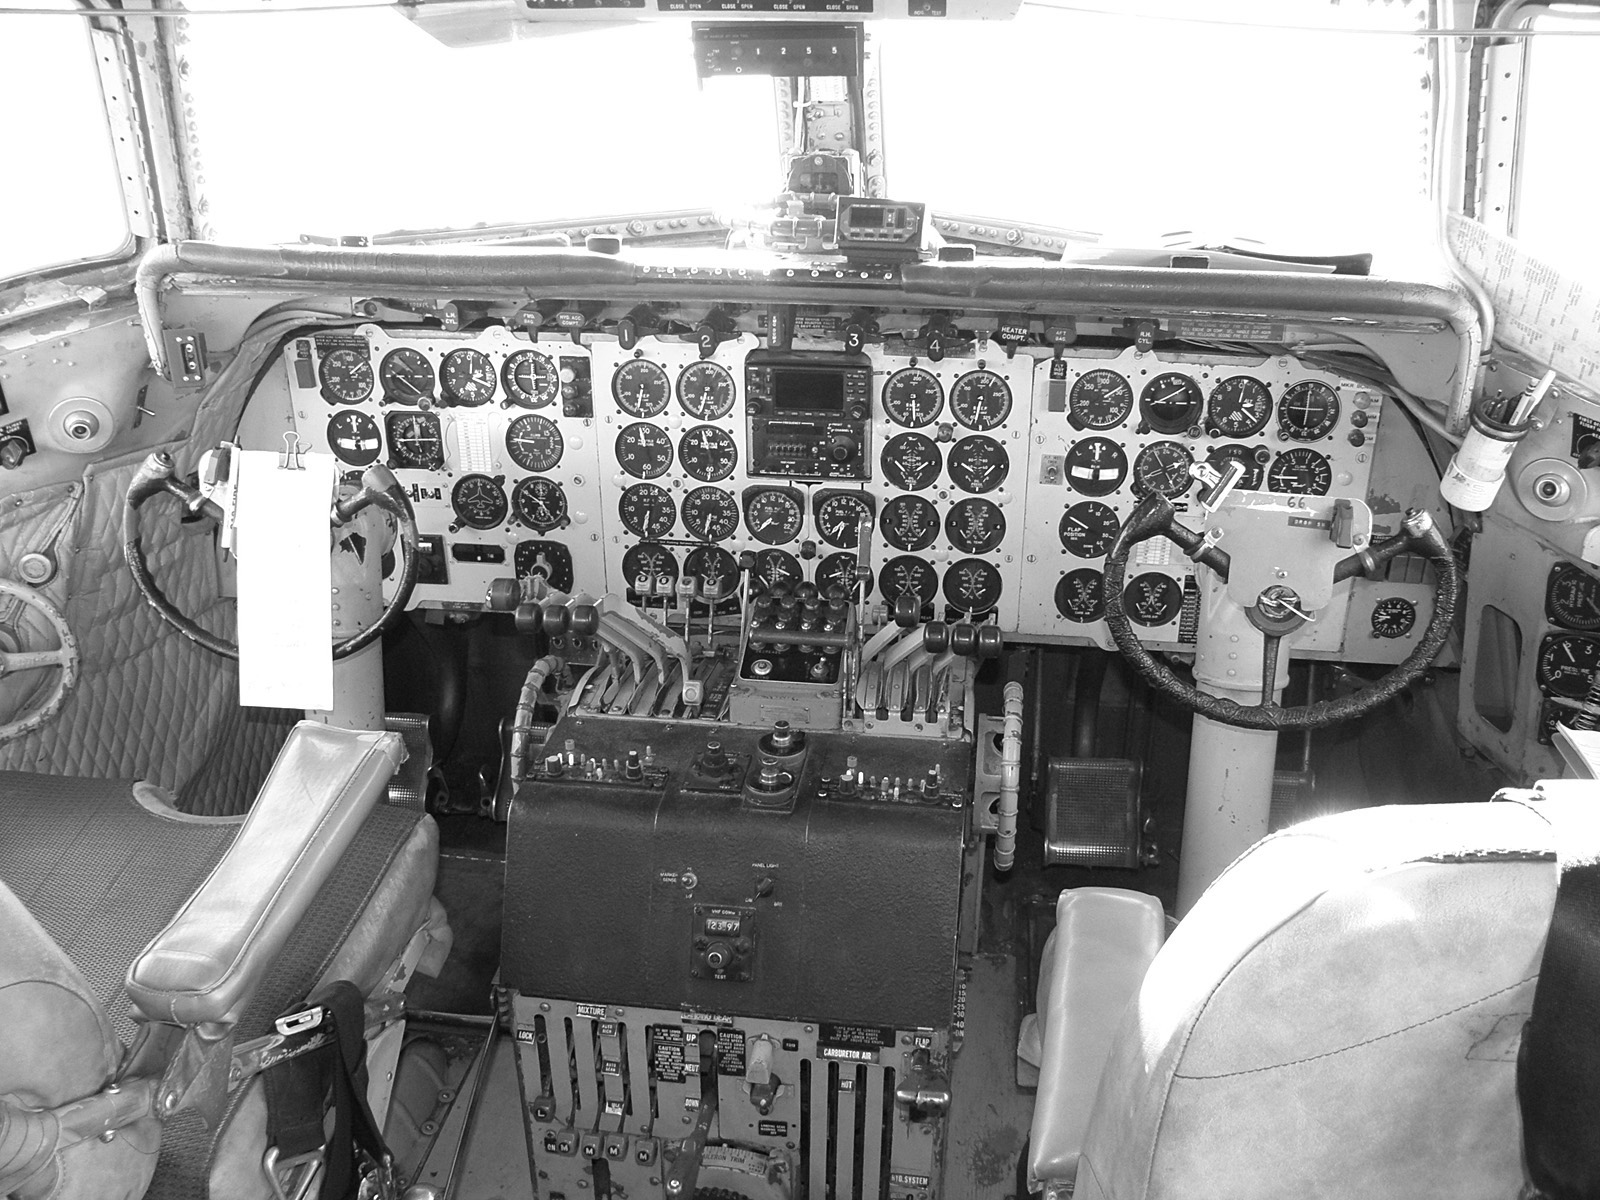
\includegraphics[width=1.6in]{images/Butler-dc7-N6353C-071102-fox-tanker66-01-16g}
\noindent
Fig.~\ref{fig:sfig}b:  DC7, 1953\cite{DC7photo}.

\end{minipage}~~~~~~\begin{minipage}{6in}


\noindent
  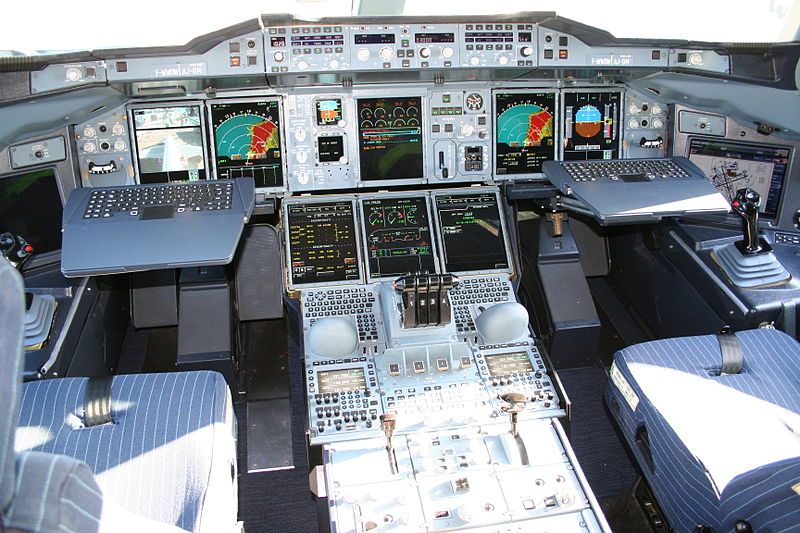
\includegraphics[width=4.8in]{images/800px-Airbus_A380_cockpit}


\noindent
Fig.~\ref{fig:sfig}c:  Airbus 380, 2005~\cite{A380Photo}.
\end{minipage}
\caption{The evolution of airplane cockpit complexity from 1936 to 2005.}\label{fig:sfig}
\end{figure*}

The algorithms behind GALE have been presented previously~\cite{krall14aaai,krallphd,galepaper}.
 Those prior reports  focused on runtimes and did not explore the analysis implications of GALE.
The core contribution of this paper is a case study on how GALE-style reasoning assists 
in the analysis of cognitive modeling.
This paper takes a large model of pilot cognition (CDA~\cite{Kim2011,Pritchett2011,Feigh2012,Kim2013,Pritchett2013}) 
and explores in detail how GALE's conclusions relate to pilot cognitive workloads and safe aircraft operation within the context of that model.
As shown in \tion{lfm}, (1)~GALE offers many novel insights into complex cognitive models; (2)~other methods would be so slow to run that it might be impractical to find those insights without GALE.


The rest of this  paper is structured as follows.
\fig{acronyms} lists the frequently used acronyms in this paper.
\tion{mot} motivates this paper with a review on how cockpits are becoming increasingly more complex. 
An effective search of the models requires the utilization of automated tools such as the multi-objective objective evolutionary algorithms (MOEAs) discussed in \tion{lfm}.
These models are intricate and take time to run. 
One such MOEA is our GALE tool discussed in \tion{cpu} which, in \tion{case} is applied to a large simulation
of pilots flying a plane.
We show that GALE can answer cognitive research questions like:
\begin{itemize}
\item RQ1:  Given a limited maximum human task load capacity, what are the effects to safety assurance when a pilot's workload exceeds his or her capacity?
\item RQ2:  What are the effects of changing how much pilots rely on automation?
\item RQ3: What are the effects of changing pilot policies for monitoring and overlooking flight procedures? 
\end{itemize}



\begin{figure}[!b]
\small\begin{tabular}{r@{~=~}l}
CDA&Continuous Descent Approach\\
CPU & Central Processing Unit\\
GALE& Geometric Active LEarning\\
HTM&Maximum Human Task load\\
MOO& Multi-objective optimization\\
WMC& Working Models that Compute
\end{tabular}
\caption{Acronyms in this paper.}\label{fig:acronyms}.
\end{figure}


\section{Motivation}\label{sec:mot}

This work is motivated by the growing complexity of  models. For example, consider a model of pilot behavior.
As shown in \fig{sfig}a, a cockpit in 1936  was little more than a starter, a yoke, a throttle, pedals, and about a dozen gauges that the pilot could use to monitor airspeed, pressures, engine speed and altitude.  
A pilot model for that kind of plane would be relatively simple.

By 1953, pilots had access to much more information.  
Civil transport aircraft now included redundant systems, including a copilot, and the other machinery as shown in \fig{sfig}b. 
Concepts of operation had to clearly define the roles and the responsibilities of the pilot and copilot. 
For these kinds of planes, pilot simulation models would be more complex.
 
By 2010, aircraft had become computers with wings; e.g. the Airbus 380 cockpit of shown in \fig{sfig}c.
Autopilots allow the pilot to turn over much of the route planning and control to automation on the flight deck, and instead pilots can now take a more passive monitoring role.
While automation has certainly helped to reduce the number of aviation accidents~\cite{Coombs2005}, the kinds of errors that lead to accidents has changed.  
In particular, as shown by the examples in \fig{accident} there have been an increasing number of accidents and of near-misses caused by the pilots' interaction with automation~\cite{Billings1991,Sarter1995,Sarter1997}.

Mitigation for human-automation interaction errors consists primarily of defining concepts of operation in which the roles and responsibilities of the pilots and of the automation are clearly laid out.
The problem here is that our current generation of cockpit systems are now so complex that, in emergency situations, misunderstandings about the current state and the most important monitoring and control tasks cause life-threatening problems.  
As a result, there is active research on using models of human-machine interaction in conjunction with model-checking in order to find these aviation cockpit (and control tower) errors at the time of automation design~\cite{Bolton2011,Rungta2013,Gelman2014}. 
Accessing the interactions between pilots and plans is a difficult task.  
Collecting enough data about pilots' behavior, repeated for an adequate sample of flight conditions, can take months to years or even decades.  
Worse, if some conclusion of that study is subsequently challenged, then it is very difficult to reproduce the conditions that led to the original conclusions.

In response to this issue, researchers have built models of behavior of humans performing in those safety critical systems.  
Using those models, analysts can quickly exercise more scenarios in a reproducible manner.  
For example, researchers at Georgia Tech~\cite{Kim2011,Pritchett2011,Feigh2012,Kim2013,Pritchett2014,Feigh2014} have developed the WMC (Work Models that Compute) framework.  
WMC's CDA (continuous descent approach) simulation models the physics of flight and the atomic actions of the pilots and the automation, in the context of prioritization schemes.

%\begin{comment} XXX
%Using
%For example, 
%CDA stands for Continuous Descent Approach.  CDA is actually an alternative approach (also called Optimized Profile Descent) %to the standard descent.  Details on that are given first in a brief background section, and then details about the model %are given thereafter.
%\end{comment}

CDA can understood by contrasting it with another landing tactic, the {\em standard descent}.  
In a standard descent, an aircraft must descend via several steps, requesting a new clearance at every step.  
As a consequence, flight times are longer and more fuel is burned.  
Also, at lower steps, the aircraft is effectively closer to the city itself, emitting lots of noise as the aircraft passes by.
As the aircraft reroutes and encircles an airport before a runway is clear to land on, these wait times equate to more noise for the city.
Additionally, it is harder to fly at lower altitudes due to changes in the atmosphere and wind environments.

By contrast a {\em continuous descent approach} is a continuous non-stepped descent in which only one request for landing is needed.  
This simplifies the communication overhead between radio towers and pilots, and avoids extended duration at low altitude.  
As a result, a continuous descent can more accurately approach the runway, less fuel is burned, and less noise is emitted into the city.  
\fig{cda_diagram} illustrates the difference between CDA and traditional landing methods.


\begin{figure}[!t]
\small
\begin{tabular}{|p{.95\linewidth}|}\hline
In the 2009 Air France 447 crash~\cite{AirFranceFinal2012}, the autopilot disengaged when it lost airspeed data from the pitot tubes.  
A copilot lost situational awareness, and believed he was in `take-off, go-around' mode, in which the appropriate response is to climb.  
However, at 38,000 feet, the rate of climb that the copilot was commanding was unsustainable; Air France 447 stalled.
During the one sequence in which the copilot responded appropriately and dropped the plane's nose, the plane gained enough airspeed that the autopilot started working again and began issuing a stall warning; this effectively punished the copilot for reacting appropriately.  
Two other, more experienced pilots on the flight deck scanned the many screens and gauges available to them, but failed to notice the fact that the copilot was commanding a climb.  
One of the pieces of data that might have helped the pilots understand their situation was the plane's angle-of-attack, but this information was available only to the automation. 

Asiana Flight 214 crashed in June of 2013 at the San Francisco International Airport (SFO).  
The final report suggests that this crash may also have been partly due to confusion about the division of labor between the pilots and the automation~\cite{AsianaFinal2014}.  
Ground automation at SFO (the precision instrument landing system) was not working, and the pilots of Asiana 214 were asked to fly a manual approach.  
The plane's tail struck the seawall at the end of the runway; the plane was too slow and too low for landing.  
Both pilots reported that, until the last few seconds of the crash, they believed the autothrottle was controlling the plane's speed.  
The autothrottle was in an `armed' position, but was not on.  The pilot flying's flight director (another system for automation in the cockpit) was \emph{deactivated} and the instructor pilot's flight director was \emph{activated}; had the systems been in the same state, the autothrottle would have `woken up'. 
The flight crew failed to monitor airspeed, and the investigators concluded that fatigue and over-reliance on automation were primary contributors to the accident.\\\hline
\end{tabular}
\caption{Two examples of accidents in which complex cockpits played a role.}\label{fig:accident}
\end{figure}




%\begin{figure*}
%  \centering
%  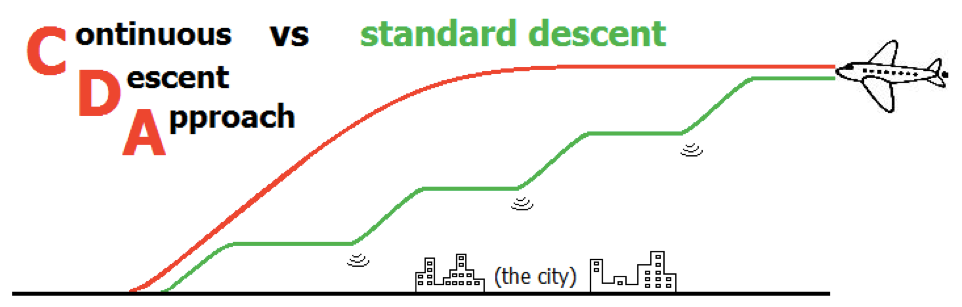
\includegraphics[width=\textwidth]{figures/cda_diagram.png}
%  \caption[Continuous Descent Approach Diagram]{Diagram of Continuous Descent Approach (CDA).  The smoother red line %represents the CDA route, while the  green stepped line represents the traditional approach.  Note that the traditional %approach is closer to the city, so the city hears the noise emitted from the aircraft, whereas the red CDA line is further %away from the city, so that there is less noise for the city.}.
%%  \label{fig:cda_diagram}
 

%CDA is made possible with satellite technology called RNP (Required Navigation Performance).  That satellite positioning %technology allows the pilot to fly the aircraft very precisely to very narrow deviation from the commanded flight course.  %Often in standard descent, the pilot will deviate off course for minutes without noticing, and the time needed to return %back on course burns extra fuel, and makes flight more expensive. 

%During approach to runway, the RNP technology allows the aircraft to precisely know where it is at, so that a stepped decent %is no longer necessary.  Without the RNP technology, the pilot would need to take smaller steps to minimize any deviations.
%As another example, consider the case where the airport is just at the base of a cliff at the south.  When the aircraft %approaches the airport from the north, traditionally, it would have to fly a huge detour around the airport and approach %from the flatter north because of the cliff.  With RNP technology for a continuous descent approach, the aircraft can %approach from the north, and descend directly despite the presence
%f the cliff.



\section{Learning From Models}\label{sec:lfm}


For analyzing complex models like CDA, we prefer GALE to traditional  optimizers since those optimizers require certain simplification assumptions.
For example, if models are simple continuous equations, then they could be readily explored with gradient descent methods such as the Quasi-Newton method (perhaps using the BFGS update rule recommended by Sims~\cite{Sims10}).
However, all such gradient descent methods assume that the model being explored is essentially continuous. 
Models like CDA are not continuous since their internal state space is divided into one combination of each branch of each {\em if statement} in the code~\cite{Davies2012}.



A better approach for exploring complex models is a multi-objective evolutionary algorithm (MOEA). 
There are many such optimizers including GALE and more traditional tools such as NSGA-II~\cite{deb00afast}.
MOEAs assume that the model is a function that converts  {\em decisions} ``$d$'' into {\em objective} scores ``$o$''; i.e.
\[
o = \mathit{model}(d)
\]
In this framework, each pair $(d,o)$ is an {\em individual} within a {\em population}. 
MOEAs try to find a range of good inputs by progressively improving the population using the {\em generational} approach of  \fig{moea}.
Note that MOEAs  make no assumptions about model continuity (e.g. unlike the Quasi-Newton methods, they do not assume that models have local smooth gradients). 
They can also explore trade-offs between goals (see the domination predicate discussed in \fig{moea}). 
As discussed below, MOEAs have problems with {\em brittleness} and {\em CPU}.


%% MOEAs approach avoids tricky problems such as local maximia 
%% via the use of random mutation (see  step 3 of \fig{moea}).
%% Also, they can be applied to models non-numeric values and non-continuous
%% internal state spaces.
%% Better yet, the {\em domination predicate} used in culling worse solutions (see step 2 of \fig{moea})
%% can  explore intricate trade-offs between competing objectives.

%% When execte
%% Learning strategies for models are search tools that require for the model to be integrated into a "MOO-format"; i.e. decisions and objectives must be defined.  The decisions are simply the inputs to the model by which the search tool attempts to make meaningful conclusions.  The objectives are outcomes from the model that are defined as goals to maximize or minimize; the search tool will then attempt to find combinations of inputs that optimize those output objectives.  Since most models are multi-objective as opposed to single-objective, there is an added challenge to optimization because typically multiple objectives conflict with each other, e.g. maximizing one objective tends to minimize another.  Hence, the ultimate goal of search tools is to discover a trade-off curve called a Pareto frontier.  For example, the green plot markers from~\fig{amus} visually shows the Pareto frontier for data regarding London Ambulance deployment.

%% \begin{figure*}
%%   \centering
%%   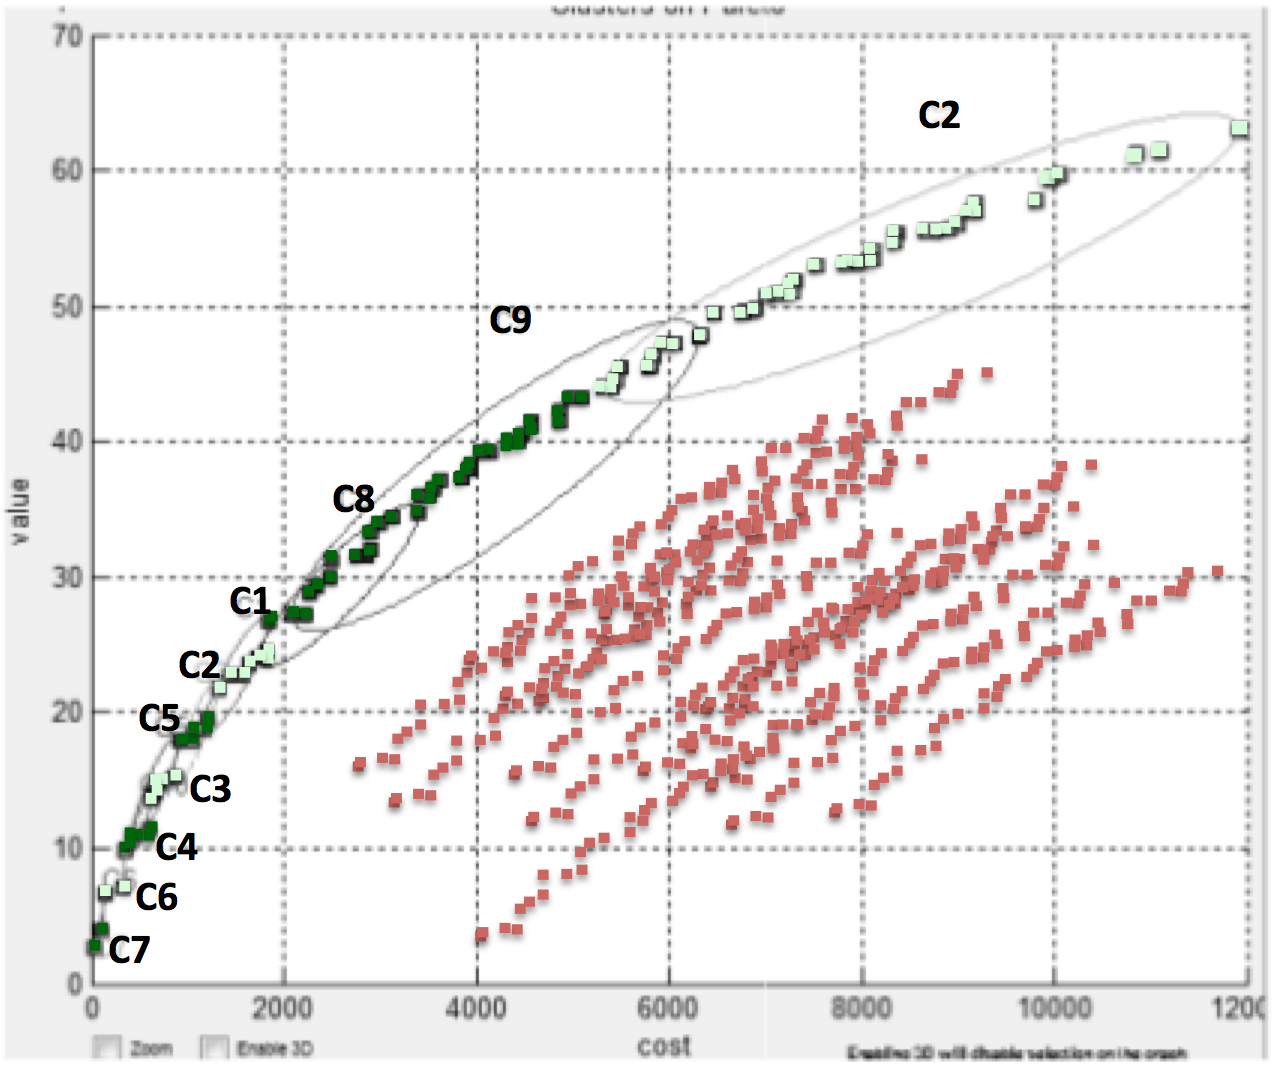
\includegraphics[width=\textwidth]{figures/amus.png}
%%   \caption{Exploring options for configuring London Ambulances~\cite{veer11} (to minimize $X$ and maximize $Y$).  An SBSE optimization algorithm has rejected thousands of options (shown in red)  to isolate clusters of better solutions C1,C2,etc (shown in green).}
%%   \label{fig:amus}
%% \end{figure*}



%% Cognitive models are meant to run more quickly than human-in-the-loop experiments, but they still take time to run.
%% The CDA model originally defined in Kim's Ph.D. thesis divides its input space 144 ways, each of which requires a separate simulation~\cite{Kim2011}. 
%% In our exploration, we further subdivide the maximum human taskload to evaluate 252
%% combinations. 
%% Worse yet, a detailed reading of Kim's thesis shows that these 144 input sets actually
%% explore only one variant each for three of her inputs~\cite{Kim2011}. 
%% Other modes would need to be explored to handle:
%% \begin{itemize}
%% \item Unpredictable rerouting;
%% \item Different tail wind conditions;
%% \item Increasing levels of delay.
%% \end{itemize}
%% If we give three ``what-if'' values to the above three items then, taken together, these 3*3*3*252 modes*inputs would require nearly 7000  different simulations.
%% This is an issue since, using standard multi-objective optimizers such as NSGA-II~\cite{deb00afast}, our models take seven hours to reach stable minima.
%% Hence, using standard technology, these 7,000 runs would take 292 weeks to complete.  
%% \ADD{Note that this complaint applies not only to NSGA-II but to all the other optimizers listed above.}


\begin{figure}[!t]
  \centering
  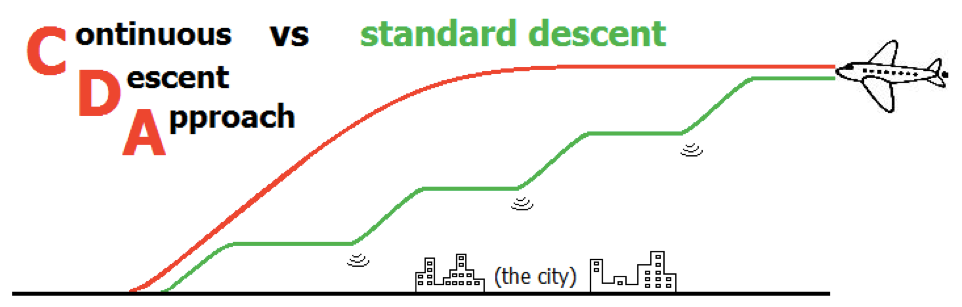
\includegraphics[width=3.5in]{figures/cda_diagram.png}
  \caption[Continuous Descent Approach]{
The red line shows a Continuous Descent Approach (CDA).
The green stepped line represents the
traditional approach, which is closer to the city,
so the city hears more noise emitted from the
aircraft.}.

  \label{fig:cda_diagram}
\end{figure}

\begin{figure}[!b]
\small
\begin{tabular}{|p{.95\linewidth}|}\hline
An evolutionary multi-objective optimization algorithm (MOEA) requires at least two  operators:
{\em cull} and  {\em perturb}:
MOEAs generate an initial population by randomly selecting decisions then {\em culling} the individuals with the lower objective scores.
A new population $P_n$ is generated by {\em perturbing}  the decisions of the surviving individuals (e.g. via random mutation or grafting together parts of the decisions of different individuals).
MOEA's halt when $P_n$ scores no better than prior generations $P_{m<n}$.


One way to implement the culling (step 2) is via {\em domination}; i.e. remove one example
if it can be shown that it is worse than (a.k.a. ``is dominated by'') some other examples. 
Two forms of domination are {\em binary} and {\em continuous} domination.
In {\em binary domination},  one individual $x$ dominates $y$ if all of $x$'s objectives are never worse than the objectives in $y$ but at least one objective in solution $x$ is better than its counterpart in $y$; i.e.
\[ \begin{array}{c}
\left\{ 
     \forall o_j  \in \textit{objectives}\;\mid\; \neg ( o_{j,x} \prec o_{j,y}) \right\} 
\\
 \left\{
\exists o_j \in \textit{objectives} \;\mid\; o_{j,x} \succ y_{j,y}\right\}
\end{array}
\]
 where ($\prec,\succ$) tests if an objective score in one individual is (worse,better) than in the other individual.

An alternate culling method is  the {\em continuous domination} predicate~\cite{Zitzler04indicator-basedselection}  that
favors $y$ over $x$ if $x$ ``losses'' least:
\begin{equation}\label{eq:cdom}
\begin{array}{rcl}
\textit{worse}(x,y)& =& \textit{loss}(x,y) > \textit{loss}(y,x)\\
\textit{loss}(x,y)& = &\sum_j^n -e^{\Delta(j,x,y,n)}/n\\
\Delta(j,x,y,n) & = & w_j(o_{j,x}  - o_{j,y})/n
\end{array}
\end{equation}
where  ``$n$'' is the number of objectives and $w_j\in \{-1,1\}$ depending on whether
we seek to maximize goal $x_j$.  
\\\hline
\end{tabular}
\caption{Multi-objective evolutionary algorithms.}\label{fig:moea}
\end{figure}
\subsection{Brittleness}

Ideally, any insight we glean from a model is not ``brittle''; i.e. it is a conclusion that is robust in the face of minor changes to model inputs.
Unfortunately, experts in MOEA reasoning caution that many MOEAs generate ``brittle'' decisions.

According to Harman~\cite{harman01}, understanding the neighborhood around individual solutions is an open and pressing issue:
\begin{quote}
 ``It may be better to locate an area of the search space that is rich in fit solutions, rather than identifying an even better solution that is surrounded by a set of far less fit solutions.''~\cite{harman04}.  
\end{quote}

He argues that many software model problems are {\em over-constrained}; i.e.  no precise solution over all variables is achievable.  
Such over-constrained problems are usually explored using heuristic search methods such as the MOEA of \fig{moea}.
The results of such partial heuristic search may be ``brittle''; i.e., small changes to the search results may dramatically alter the effectiveness of the solution~\cite{harman04}.  
 One way to check for brittleness is to use {\em neighborhood perturbation}:
\begin{enumerate}
\item {\em Cluster}  a  population into local neighborhoods;
\item  Build a new population by {\em perturb}ing the decisions in each neighborhood;
\item Halt if objectives do not change after perturbation;
\item Else, go to step 1.\end{enumerate}
One reason we endorse the GALE algorithm for reaching conclusions from complex cognitive models is that it directly implements neighborhood perturbation.



\subsection{Problems with CPU}\label{sec:cpu}
CDA is a complex model with many input parameters. 
The input parameter space for such models tends to grow very large so there is a pressing and urgent need for efficient modeling techniques.

The primary design criteria for standard MOEAs is ``ability to explore complex trade-offs'' and not runtime speed.
While the internal details of standard MOEAS may be very different (see \fig{sample}); most of them share one key characteristic:
they evaluate $O(2N)$ examples (twice the population size because they generate offspring which are perturbations of their parent examples) for each generation.  One reason we advocate GALE is that it replaces
 $O(2N)$ with a much faster $O(log_2N)$ technique (see below).


\begin{figure}
\begin{tabular}{|p{.95\linewidth}|}\hline
\small
\bi
\item NSGA-II~\cite{deb00afast} 
uses a non-dominating sort procedure to divide the solutions into {\em bands} where {\em band}$_i$ dominates all of the solutions in {\em band}$_{j>i}$ (and NSGA-II favors the
least-crowded solutions in the better bands).
\item
{\em SPEA2}: favors solutions that dominate the most number of other solutions that are not nearby (to break ties, it uses density sampling)~\cite{zit02}; 
\item {\em  IBEA}:
uses continuous dominance to find the solutions that dominate all others~\cite{Zitzler04indicator-basedselection}; 
\item In {\em Particle swarm optimization} (PSO), a {\em particle}'s velocity is `pulled' towards the individual and the community's best current solution~\cite{pan08};
\item 
The {\em many-objective optimizers} are designed for very large numbers of objectives~\cite{deb14}; 
\item
Multi-objective {\em differential evolution} (DE): members of the frontier compete (and are possibly replaced) by candidates generated by extrapolation from any three other members of the frontier~\cite{storn97,5601760};
\item
The {\em decomposition methods} that {\em first} divide the space of candidate solutions into numerous small regions; then {\em second} run a relatively simple optimizer in
each region~\cite{deb05,zhang07}.
\ei \\\hline
\end{tabular}
\caption{Some sample MOEAs. Note that this list is not exhaustive since this is a very active area of research.}\label{fig:sample}
\end{figure}


\begin{figure}
\small
\begin{tabular}{|p{.95\linewidth}|}\hline
GALE initially builds a population of points by selecting
decisions at random. 
It then {\em clusters} those decisions into neighborhoods as follows:
\begin{enumerate}
\item
Find two distant points in that population; call them the {\em east} and {\em west} poles. 
\item 
Draw an axis of length $c$ between the poles. 
\item
Let each point be at distance $a,b$ to the {\em east, west} poles.
Using the cosine rule, project each point onto the  axis  at $x=(a^2 + c^2 - b^2)/(2c)$.  
\item 
Using the median $x$ value, divide the population.
\item
For each half that is larger than $\sqrt{N}$ of the original population, go to step 1.
\end{enumerate}
Note that the above requires a distance measure between sets of decisions: GALE uses the standard case-based reasoning measure defined by Aha et al.~\cite{aha91}. 
Note also that GALE implements step 1 via  the FASTMAP~\cite{Faloutsos1995} linear-time heuristic:
\begin{itemize}
\item
Pick any point at random; 
\item Let {\em east} be the point furthest from that point; 
\item Let {\em west} be the point furthest from {\em east}.
\end{itemize}
These final sub-divisions found by this process are the {\em neighborhoods} that
GALE will {\em perturb} as follows:
\begin{itemize}
\item
Find the objective scores of the {\em east, west} poles in each neighborhood.
\item 
Using the continuous domination predicate of \fig{moea}, find  the {\em better} pole. 
\item
Perturb all points in that neighborhood by pushing them towards the better pole, by a distance  $c/2$ (recall that  $c$ is the distance between the poles).
\item
Let generation $i+1$ be the combination of all pushed points from all neighborhoods.
\end{itemize}
From a formal perspective, GALE is an active learner~\cite{Dasgupta2005} that builds a piecewise linear approximation to the Pareto frontier~\cite{Zuluaga:13}.
For each piece, it then pushes the neighborhood up the local gradient.
This  approximation is built in the reduced dimensional space found by the FASTMAP  Nystr\"om approximation to the first component of PCA~\cite{platt05}.
\\\hline
\end{tabular}
\caption{Inside GALE}\label{fig:gale}
\end{figure}

GALE combines (a) the neighborhood perturbation (described above) with (b)~the MOEA algorithm of \fig{moea}.
The algorithm reflects over a {\em population} of points, each of which contains {\em decisions} (some inputs to a  model).
It then searches for the input decisions that lead to best outcomes.
For example:
\begin{itemize}
\item
if we adjust the inputs to the model for (say) high tailwind conditions...
\item
... then GALE can report the best monitoring policies for the cockpit instrumentation.
\end{itemize}

\fig{gale} lists the procedure by which GALE clusters the data into neighborhoods, then perturbs each neighborhood.
In terms of monitoring for brittleness, the key point of GALE is that  this process continues until the perturbations stop having any new effect (i.e. they stop generating better objective scores). 
That is, all GALE solutions are guaranteed not to be brittle.


Also, in terms of reducing runtime, the key feature of GALE is that, unlike traditional MOEAs such as NSGA-II~\cite{deb00afast}, GALE does not evaluate its entire population.
Instead, as it recursively clusters the data in two (using steps 1,2,3,4,5 in \fig{gale}), GALE only computes the objective scores for the two most distant points in each division.  
This means that this binary division of the data terminates after just $log_2(N)$ comparisons of evaluated individuals. 
This is much less than the $2N$ evaluations required by  traditional methods like NSGA-II.

Note that the above is a very brief description on GALE. For a full description including algorithms, download sites, and results
from dozens of models, see \cite{galepaper,krallphd}.

\section{A Case Study:  CDA and GALE}\label{sec:case}

This case study was designed after reflecting on the following.
Sometimes, when monitoring cockpit instruments, a pilot is unable to complete all of their required tasks.
Such lack-of-attention can have adverse consequences on aviation safety.
It can occur for many reasons, including (1)~fatigue; or
(2)~unexpected or stressful situations such as:
\bi
\item 
Unexpected flight conditions such as increased tail winds or unscheduled rerouting;
\item
Emergency situations (e.g. a threatened near miss with another aircraft);
\item
Training situations in which one pilot must monitor a plane at the same time as watching over another, less experienced, pilot.
\ei
\subsection{Goals}

The goals of this study are:
\be
\item
To understand the safety implications of lack-of-attention;
\item
To learn what mitigations exist (if any) for reducing safety problems associated with lack-of-attention.
\ee
\ADD{We use interrupted, forgotten, and delayed tasks within the CDA model as an incomplete proxy for a safety metric.
Our possible mitigations are restricted to the input of our CDA problem space.}


\subsection{Methods}
\subsubsection{Apparatus}

This study uses the CDA model as described herein. 
CDA is a model of pilot interactions: with each other and also with the navigation systems critical to safe flight.  
CDA employs a continuous descent approach to a runway. 
As aforementioned, a continuous descent is an alternative to the standard approach to a runway.
A continuous descent approach is arguably much more efficient in terms of a) fuel economy and cost, b) noise, and c) flight duration.

CDA is packaged within the WMC (Work Models that Compute) suite.  
%WMC is a tool that was used to generate the CDA model.  
%This functionality is useful in human factors analysis because 
WMC has the capability of modeling the way humans select which task to do next.
In the CDA model, pilots have a handful of requirements and tasks that they must satisfy, and each requirement and task has a given level of priority that affects the order in which it is satisfied.
WMC also takes into account that humans have a ``maximum human task load" variable which describes how much they can handle.  
If the task load is too large, then some of the workload will not be completed in time, or worse yet, might go forgotten entirely.  
We use the metrics that describe these problems as the output objectives for GALE, i.e., the dependent variables which are detailed in the subsection just below.

Different strategies of pilot interaction can help alleviate the problems of large task loads.  These different strategies are employed in CDA through its inputs, i.e. the independent variables as described in the next subsection.  
By studying the different strategies in terms of the output objective scores (the dependent variables), it is possible to understand the safety implications of different strategies and to learn what mitigations might exist (and can be exploited for safety gain).


\subsubsection{Independent Variables}

A CDA ``problem instance'' defined within the WMC framework consists of four decisions and five objectives.  
The CDA implementation itself within WMC contains many other inputs (for example, the flight path and aircraft type are fixed) but for the purposes of this study, they are held constant. 


%\begin{changed}
%\begin{enumerate}
%\item \textbf{HTM}: maximum human task load. This value describes how many tasks (where a task is an atomic action) can be maintained in a mental to-do list by a person.  Tasks in the model are assigned a duration and a priority. For a thorough description of this variable, please see~\cite{Kim2011}. When the number of necessary tasks exceeds the number of tasks that the person can maintain, there can be incurred delays, errors, or the possibility of the task being forgotten and lost.
%\item \textbf{FA}: function allocation.  This variable refers mainly to the relative authority between the human pilot and the avionics, and is discussed in more detail to follow.
%\item \textbf{CCM}: contextual control mode of pilots. These describe the pilots' ability to apply patterns of activity in response to the demands and resources in the environment, and are described in detail below.;
%\item \textbf{SC}: the  air environment  scenario.  WMC's CDA model includes four different arrival and approach scenarios.
%\end{enumerate} 
%\end{changed}
CDA's four decision variables are:
\begin{description}
\item[HTM:] maximum human task load. This value describes how many tasks (where a task is an atomic action) can be maintained in a mental to-do list by a person.  Tasks in the model are assigned a duration and a priority. For a thorough description of this variable, please see~\cite{Kim2011}. When the number of necessary tasks exceeds the number of tasks that the person can maintain, there can be incurred delays, errors, or the possibility of the task being forgotten and lost.
\item[FA:] function allocation.  This variable refers mainly to the relative authority between the human pilot and the avionics, and is discussed in more detail to follow.
\item[CCM:] contextual control mode of pilots. These describe the pilots' ability to apply patterns of activity in response to the demands and resources in the environment, and are described in detail below.;
\item[SC:] the  air environment  scenario.  WMC's CDA model includes four different arrival and approach scenarios.
\end{description} 

%\begin{changed}
%   \be
%   \item{\em Nominal} (ideal) arrival and approach.
% \item{\em Late Descent}: controller delays the initial descent.
% \item{\em Unpredicted rerouting}:  pilots  directed to an unexpected waypoint.
%\item{\em Tailwind}: wind  pushes  plane from  ideal trajectory.
%\ee
The four arrival and approach \emph{scenarios} (SC) implemented within the CDA model are:    
\begin{description}
\item[Nominal:] (ideal) arrival and approach.
\item[Late Descent:] controller delays the initial descent.
\item[Unpredicted rerouting:]  pilots  directed to an unexpected waypoint.
\item[Tailwind:] wind  pushes  plane from  ideal trajectory.
\end{description} 
The {\em function allocation} (FA) defines the different ways the pilots can configure the autoflight controls.  We list the different possible modes within the CDA below, interested readers are referred to~\cite{Pritchett2014} for more details.
\begin{description}
\item[Highly Automated:] The computer processes most of the flight instructions directly; the pilot only confirms the clearances.
\item[Mostly Automated:] The pilot processes the instructions and programs the autoflight sytem, but then the autoflight system controls the flight path automatically.  This mimics current ``LNAV" and ``VNAV" flight operations.
\item[Mixed-Automated:] The pilot processes the instructions and programs the computer to handle the lateral flight path. The flight crew directly flies the vertical profile, including the altitude, vertical speed, and airspeed.
\end{description} 
%    \be
 %   \item{\em Highly Automated:} The computer processes most of the flight instructions directly; the pilot only confirms the clearances.
 %   \item{\em Mostly Automated:} The pilot processes the instructions and programs the autoflight sytem, but then the autoflight system controls the flight path automatically.  This mimics current ``LNAV" and ``VNAV" flight operations.
 %   \item{\em Mixed-Automated:} The pilot processes the instructions and programs the computer to handle the lateral flight path. The flight crew directly flies the vertical profile, including the altitude, vertical speed, and airspeed.
%    \ee
CDA also knows of three different pilot {\em contextual control modes} (CCM).  These are based on Hollnagel's work on representative patterns of activity~\cite{Hollnagel1993}. For more information on how these CCM's are implemented as sets of actions within WMC, please refer to~\cite{Feigh2014}.
\begin{description}
    \item[Opportunistic:]  Pilots monitor and perform tasks related to only the most critical functions.
    \item[Tactical:] Pilots cycle through most of the available monitoring tasks, and double check some of the computer's tasks.
    \item[Strategic:] Pilots cycle through all of the available monitoring tasks, and try to anticipate future tasks.
\end{description} 
%    \be
 %   \item{\em Opportunistic}:  Pilots monitor and perform tasks related to only the most critical functions.
 %   \item{\em Tactical}: Pilots cycle through most of the available monitoring tasks, and double check some of the computer's tasks.
  %  \item{\em Strategic}: Pilots cycle through all of the available monitoring tasks, and try to anticipate future tasks.
  %  \ee
%\end{changed}


\subsubsection{Dependent Variables}

CDA's five objectives  keep track of how many tasks were delayed, interrupted or forgotten entirely (which impacts the relative safety of the flight itself).  
We summarize these metrics below; the interested reader should see~\cite{Kim2011} for full details. 
Better pilot organizational structures can be found by exploring different inputs of CDA to optimize these goals so that safety is improved:
\begin{description}
\item[Num Forgotten Actions:] tasks forgotten by the pilot. When the number of tasks expected of the pilot exceed the HTM, tasks with the lowest priority are `forgotten'.
\item[Num Delayed Actions:] number of delayed actions. Tasks have a scheduled time and a duration.  When a higher priority task causes another task to begin later than its scheduled time, it is `delayed'.
\item[Num Interrupted Actions:] interrupted actions. A higher priority task can cause a lower priority task to be interrupted.
\item[Interrupted Time:] time spent on  interruptions.
\item[Delayed Time:] total time of all of the delays.
\end{description}
%\begin{changed}
%\be
%\item \emph{Num Forgotten Actions}: tasks forgotten by the pilot. When the number of tasks expected of the pilot exceed the HTM, tasks with the lowest priority are `forgotten'.
%\item {\em Num Delayed Actions}: number of delayed actions. Tasks have a scheduled time and a duration.  When a higher priority task causes another task to begin later than its scheduled time, it is \em{delayed}.
%\item  \emph{Num Interrupted Actions}: interrupted actions. A higher priority task can cause a lower priority task to be interrupted.
%\item  {\em Interrupted Time}: time spent on  interruptions.
%\item \emph{Delayed Time}: total time of all of the delays.
%\ee
%\end{changed}

In CDA, the HTM (maximum task load) variable controls how many tasks a pilot can either perform or hold in working memory.
In all the following, CDA was run for varying and decreasing values of HTM.
For each HTM value, we collect:
\bi
\item {\em The  baseline objective scores} seen in CDA. Recall from the above that those baseline values relate to number of
forgotten actions; delayed actions; interrupted actions;
total interrupted time; etc.
\item {\em The treated objective scores} seen in CDA. These treatments are learned
by GALE and represent the best case actions that could be performed by pilots
to mitigate against the lack-of-attention problem.
\ei

When analyzing CDA, GALE was run using  parameters found to work best on several other models~\cite{krallphd}:
\bi
\item GALE uses a population of size 100;
\item GALE must  terminate after a maximum number of 20 generations;
\item GALE may terminate if no improvement is seen in any objective in the last three generations;
\ei
To control for random effects during optimization, all scores are the mean values of 20 repeated runs of {\em baseline} or  the model {\em treated} with GALE's conclusions.

\subsubsection{Data Analysis}
Originally, we only planned one experiment, called {\em Experiment \#1},  to compare {\em baseline} and {\em treated} by letting GALE select any inputs across the full range of all CDA input values.

\begin{changed}
That first experiment found a curious threshold effect: underneath a certain HTM point, all the best decisions concerned a particular contextual control mode.  
As described above, in {\em Opportunistic} mode, pilots monitored and performed tasks related to only the most critical functions in the cockpit. 
That is, in this mode, pilots executed only the most essential monitoring actions according to the CDA model (e.g. monitoring altitude and monitoring descent airspeed), and focused primarily on adjusting the lateral profile.  For full details, see~\cite{Kim2011}, pages 110-135.
\end{changed}

To  understand the impact of this {\em Opportunistic} mode, an {\em Experiment \#2} was conducted, exactly like Experiment \#1, but with the {\em Opportunistic} mode  disabled.

\subsubsection{Sanity Checks}
We define two  sanity checks on our results:

{\em Sanity check \#1:}
The clear pre-experimental intuition is that, as we 
{\em decrease}
HTM (maximum human task load), we should see {\em increasing} adverse flight operations. 
If this observation was not seen in the results, the entire investigation should be doubted.

{\em Sanity check \#2:} Using CDA and GALE, we can find mitigations that reduce the effects of decreasing HTM. 
If this were otherwise, that would suggest that MOEAs like GALE are not useful here.



%% To expand on that last problem, Krall comments~\cite{krallphd} that models can be very slow to optimize even if the model just a few hundred milliseconds per run.  The CDA model requires about 6-8 seconds of runtime per run, so that last problem can become a very serious issue (and it is).  Thousands of runs at those runtimes can take several hours, and worse yet, engineers at NASA Ames want to repeat this process for hundreds of different scenarios (different tailwind conditions; different frequencies of how often ground control demands course changes, etc).  It is estimated that by using standard methods, and running on one CPU (as opposed to parallel processing), that those runs would take six years of calendar time to complete.

%% Although possible to reduce that runtime complexity with parallel processing, recently in~\cite{galepaper}, Krall et al. have been exploring a more efficient approach to reduce the number of model runs, called GALE (Geometric Active Learning Evolution).  Standard tools take a Monte Carlo approach to studying complex models.  That approach requires generating populations (of size $N$) of candidate inputs to the model, and then in each iteration of the tool, running the model $2N$ times (an $O(2N)$ order of complexity).  The data mining approach of GALE on the other hand, analyzes the input population structure to find the most informative subsets of candidates, and only runs the model with those selected candidates (which number just a few dozen, usually).  Thus, GALE only requires at most $2log_2(N)$ model runs per iteration, and usually requires fewer iterations that Monte Carlo methods as well.

%% GALE is essential for the task at hand in this paper.  Previously in~\cite{krall14aaai}, GALE was compared to standard methods that took 3-5 hours per run whereas GALE only needed 6-20 minutes; that study was only for one single mode of CDA.  In this paper, 16 different modes of CDA are explored.  It would require a year of calendar time alone just to explore CDA with two other standard methods.  GALE on the other hand reduces that time requirement to 83 hours, a reduction factor of just over 100 times less.

%% This paper stresses that the contribution here is not GALE, but rather the methodology in approaching cognitive studies for aircraft research.  Previously in~\cite{krall14aaai}, a subset of this paper appeared and only one mode of CDA was explored.  This paper is an extension of that previous work which explores many more models as made possible only through the application of GALE. 

%% The key takeaways from this paper are a follows.  A
%% trend in the cognitive limitations of pilots has
%% been identified.  In that trend, whenever cognitive
%% limits have been exceeded, the key is to let
%% automation take over most of the operation.
%% \todo{misty can comment on these next statements ->}
%% Much of the aircraft operations community has
%% commented on the effect of over-reliance of falling
%% back on automated operations.  If pilots often
%% switch to automated modes during off-nominal
%% situations, then they do not receive the training
%% and experience necessary in the case when automated
%% modes are disabled or non-operational.  Poorly
%% trained pilots in those cases have been the subject
%% of many safety failures and disasters in the past.
%% Hence, the identification of this trend may be an
%% alarming one to the community: humans should be the
%% last fail-safe during flight operations.  This line
%% of thought is elaborated in the next section on
%% motivation and related work.




%% Much of the MOO literature has focused on optimizing simple math models, such as Fonseca~\cite{Fonseca95anoverview}, Schaffer~\cite{Schaffermodel}, Osyczka2~\cite{osymodel} and many others, which consist of simple mathematical transformation functions (which map independent variables to dependent variables, i.e. the inputs and outputs) as opposed to complex algorithms for simulation.  Conceptually, there is no difference in technique for optimizing those models.  However, math models are extremely fast to evaluate and inputs can be mapped to outputs in less than a millisecond as opposed to several seconds.  Hence, much of the MOO literature was able to run the models as often as possible with no penalty to the overall runtime for learning.  In other models where the behavior cannot be modeled via math, the model evaluation-times are often hundreds of milliseconds to several seconds long.  Thus, the search tools that typically evaluate the model thousands to millions of times can incur very large penalties to runtime.  For CDA, which is several seconds long, it is not possible to evaluate thousands of times unless thousands of processor hours are available to exploit - even so, lengthy runtimes can be impractical to work with.

%% Recently, we have been exploring a data mining approach to search tools which evaluates the model far fewer times than the standard methods, called GALE (Geometric Active Learning Evolution)~\cite{galepaper},\cite{krallphd}.  
%% Whereas standard methods employ a Monte Carlo method for random search, GALE applies data mining techniques that analyze the structure of the data before selecting just a few candidates to evaluate as the basis of reasoning.

%% \subsection{GALE}

%% GALE stands for Geometric Active Learning Evolution and it is an evolutionary multi-objective optimization algorithm (EMOO, or MOEA).  MOEAs employ population management techniques to first generate a completely random initial population (of size $N$).  The members of the population are "candidates" which consist of possible inputs to the model being optimized.  When that candidate sends its inputs to the model for evaluation, that candidate acquires its fitness score which consists of the objective outputs from the model running on those inputs.

%% Standard MOEA tools are stochastic search methods which explore the input space randomly in search of inputs which optimize the objectives.  Two of the most popular MOEA tools are NSGA-II~\cite{deb00afastafast}, and SPEA2~\cite{zit02} (according to Ammar and Sayyad~\cite{sayyad13c}).  Those two search tools are much like any other search tool from the literature and they require $2N$ evaluations per iteration (an "evaluate everyone" policy).  That number is twice the population size because MOEA tools generally "reproduce" by creating an offspring population which is mutated and passed through biologically-inspired crossover and mutation operators.  To manage the population and retain its size, both the parent and offspring populations are evaluated in order to "sort" (the main feature for NSGA-II and SPEA2), the population and cull the least desired (worst fitness) members.  MOEA tools repeat this process for a number of iterations until some stopping criteria tells the tool to stop.  

%% GALE, on the other hand, is a much faster technique which applies data mining techniques to analyze the population of candidates (in its input space) to cluster them and select a small subset of the most interesting candidates.   Those candidates are then mutated directionally (as opposed to randomly) in a desirable direction.  The end result is that GALE requires only $2Log_2(N)$ evaluations per iteration.  In this section, only a very high level overview of GALE was given.  In the next section, GALE is detailed on an algorithmic level and pseudo-code is also given.  

%% \subsection{Further Technical Details for GALE}

%% GALE combines \emph{active learning}, \emph{spectral learning} and \emph{directed mutation} into search:

%% \begin{itemize}
%% \item Active Learning is an umbrella term for learning the most from using the least.  In Machine Learning, the labeling of data (such as evaluating candidates) is an expensive operation and the aim is to reduce the number of labeling operations performed~\cite{Dasgupta_atutorial}.  In theory, labeling subsets of the data may yield performances that are just as good (or close to) as labeling the entire dataset.  Hence, active learning seeks to find minimal subsets that yield maximal performance results.  Active Learning has previously been applied to MOEAs in~\cite{Zuluaga:13} to reduce the number of required evaluations of the search tool, however their algorithm is complex to understand and involves the use of Gaussian Processes to predict evaluation outcomes.
%% \item Spectral learners re-express $d$-dimensional data in terms of the $e$ eigenvectors of that data.
%% That is, raw dimensions are expressed in terms of the spectral dimensions~\cite{KamvarKM03}.  The spectral dimensions offer more meaningful information; they describe the variance in the data.  To obtain those spectral dimensions however, an expensive $O(n^3)$ operation can make spectral learners very slow for larger datasets.
%% To offset that, the Nystrom Method~\cite{nystromoriginal} is used to find a lower-rank approximation of the dataset.  While Spectral Learning has a wide-application radius~\cite{Cortes09learningnonlinear},\cite{Fine:2002:EST:944790.944812},\cite{_sparsekernel},\cite{JMLR:v14:talwalkar13a}, the specific field of interest for GALE is Spectral Clustering, as in~\cite{FowlkesBCM04},\cite{Ng01onspectral}, \cite{BachJordan2003}. 
%% \item Directed Mutation is an approach to perturbing candidates from populations of a MOEA search tool.  Typical stochastic methods use standard mutation (as biologically inspired) to randomly change the candidate.  Random mutation can generate poor candidates and only a few strong candidates.  Instead of mutating randomly, a directed approach first approximates a preferred direction for mutation and then directs candidates in that direction for improvement.
%% \end{itemize}

%% GALE begins with an initial population which is randomly generated.  In its iterative phase, that population is clustered via the WHERE~\cite{me12d} spectral learner.  WHERE clusters the population via a recursive descent approach similar to Boley's Principal Direction Divisive Partitioning (PDDP) algorithm~\cite{boley98}.  PDDP finds principal components (e.g. the directions of most variance, e.g. the spectral dimensions) and splits the data in half along the first principal component.  The WHERE tool is different than PDDP in that WHERE uses a Nystrom Method to simplify the operation to find principal components.  For each half of the split, the procedure is repeated until the parts are within some threshold; the parts are then called leafs.

%% An important detail of WHERE is in the Nystrom Method used; elements of the dataset are projected onto just the first principal component via the FastMap tool~\cite{Faloutsos1995}, (Platt certifies that FastMap is a Nystrom method~\cite{Platt05fastmap}); as such, FastMap is a tool with near-linear complexity as opposed to a tool with cubic complexity.  To see just how simple FastMap is, the lines below summarize the algorithm:

%% \bi
%%   \item Given a population of data points,
%%   \item Pick any point $x$ at random.
%%   \item Let {\em east} be the furthest point from $x$.
%%   \item Let {\em west} be the furthest point from {\em east}.
%%   \item Let the line ($east$, $west$) be the first spectral dimension. 
%% \ei

%% All the data points are then projected onto that first spectral dimension via a law of cosines that maps the point directly to the line to form a right-angle between it and the line:

%% \bi
%% 	\item For each point, x\footnote{x (and any other point) is a vector of dimension n, where n is the number of inputs to the model being optimized}
%% 	\item Let $a = dist(x, east)$
%% 	\item Let $b  = dist(west, x)$
%% 	\item Let $c = dist(east, west)$
%% 	\item $x' = (a^2 + c^2 - b^2)/(2c)$
%% \ei

%% Active learning comes into play during FastMap: only the $east$, $west$ pairs of data points are evaluated.  After WHERE splits the line between $east$, $west$ in half, only one half is further explored (unless WHERE is run without pruning).  Reducing the number of evaluations in GALE is key, so WHERE is run with pruning.  The half which is suppressed from further exploration is the half containing the one of $east$,$west$ which is a weaker candidate (according to its fitness).  To determine which of $east$,$west$ is the weaker candidate, \emph{Continuous Domination}\footnote{For details on Continuous Domination, refer to section 3.1 of Zitzler \&  K\"unzli for their IBEA algorithm~\cite{Zitzler04indicator-basedselection}.} is used to calculate an overall "loss in quality" between the pair of points and the point which losses the least is preferred as the stronger candidate.

%% To visualize the WHERE tool,~\fig{cluster1} demonstrates the recursive division of 400 instances of data; in the first part of that figure, all halves of the data are explored like a complete binary tree.  In the other part of that figure, the exploration of some halves are suppressed and fewer leafs are returned.  Overall pseudo-code of WHERE is given in~\fig{whereCode}. 


%% \begin{figure}[!t]
%% {\fontsize{2mm}{0em}\selectfont 
%% ~~~~~~~~\begin{minipage}[t]{1.5in}
%% {\small 
%% {\bf Figure4a:} 
%% Dividing 400 instances using just the independent variables.}

%% \begin{verbatim}
%% 400
%% |  > 200
%% |  |  > 100
%% |  |  |  > 50
%% |  |  |  |  > 25
%% |  |  |  |  < 25
%% |  |  |  < 50
%% |  |  |  |  > 25
%% |  |  |  |  < 25
%% |  |  < 100
%% |  |  |  > 50
%% |  |  |  |  > 25
%% |  |  |  |  < 25
%% |  |  |  < 50
%% |  |  |  |  > 25
%% |  |  |  |  < 25
%% |  < 200
%% |  |  > 100
%% |  |  |  > 50
%% |  |  |  |  > 25
%% |  |  |  |  < 25
%% |  |  |  < 50
%% |  |  |  |  > 25
%% |  |  |  |  < 25
%% |  |  < 100
%% |  |  |  > 50
%% |  |  |  |  > 25
%% |  |  |  |  < 25
%% |  |  |  < 50
%% |  |  |  |  > 25
%% |  |  |  |  < 25
%% \end{verbatim}
%% \end{minipage}~~~~~~~~~\begin{minipage}[t]{1.5in}
%% {\small
%% {\bf Figure4b}: Dominated sub-trees are pruned via active learning techniques.}

%% \begin{verbatim}
%% 400           
%% |  > 200  <-- pruned
%% |  < 200 
%% |  |  > 100 
%% |  |  |  > 50 <-- pruned
%% |  |  |  < 50 
%% |  |  |  |  > 25 <-- pruned
%% |  |  |  |  < 25 
%% |  |  < 100 
%% |  |  |  > 50 
%% |  |  |  |  > 25 
%% |  |  |  |  < 25 
%% |  |  |  < 50 
%% |  |  |  |  > 25 
%% |  |  |  |  < 25 
%% \end{verbatim}
%% \end{minipage}}
%% \caption{Recursive division via WHERE of 400 instances 
%% (using FastMap).}\label{fig:cluster1}
%% \end{figure}

%% \lstset{
%%    language=Python,
%%     basicstyle=\ttfamily\fontsize{2.7mm}{0.8em}\selectfont,
%%     breaklines=true,
%%     prebreak=\raisebox{0ex}[0ex][0ex]{\ensuremath{\hookleftarrow}},
%%     frame=l,
%%     showtabs=false,
%%     showspaces=false,
%%     showstringspaces=false,
%%     keywordstyle=\bfseries,
%%     emph={furthest,gale,better,improved,where,fastmap,split,project,mutate,mutate1}, emphstyle=\bfseries\color{blue},
%%     stringstyle=\color{green!50!black},
%%     commentstyle=\color{gray}\itshape,
%%     numbers=left,
%%     captionpos=t,
%%     escapeinside={\%*}{*)}
%% }

%% \begin{figure}
%% \begin{lstlisting}[mathescape,frame=l,numbers=left]
%% def where(data, scores={}, lvl=10000, prune=True):  
%%   "Recursively split data into 2 equal sizes."
%%   if lvl < 1: 
%%      return data # stop if out of levels
%%   leafs      = [] # Empty Set
%%   left,right = fastmap(data)
%%   west, east = data.poles
%%   $\omega=\sqrt{\mu}$ # enough data for recursion
%%   goWest = len(left) > $\omega$  
%%   goEast = len(right) > $\omega$ 
%%   if prune: # if not pruning, ignore this step
%%     if goEast and better(west,east,scores): 
%%        goEast = False 
%%     if goWest and better(east,west,scores): 
%%        goWest = False 
%%   if goWest:  
%%      leafs += where(left,  lvl - 1, prune)  
%%   if goEast:  
%%      leafs += where(right, lvl - 1, prune) 
%%   return leafs

%% def better(x,y,scores):
%%    "Check if not worse(y,x) using continuous domination. If any"
%%    "new evaluations, cache them  in 'scores'."
%% \end{lstlisting}
%% \caption[WHERE Pseudo-code]{Active learning in GALE:
%% recursive division of the data;
%% only evaluate two distant points in each cluster;
%% only recurse into non-dominated halves.
%% In this code, $\mu$ is size of the original data set.
%% }
%% \label{fig:whereCode}   
%% \end{figure}


%% GALE applies WHERE in each iteration to select just a few leafs containing the most interesting subset of the data.  The members of those leafs are then directionally mutated towards (or beyond) the stronger of $east$,$west$ in that leaf, as summarized in~\fig{mutantCode}.  Overall GALE pseudo-code is given in~\fig{galeCode}.

%% \begin{figure}
%% \begin{lstlisting}[mathescape,frame=l,numbers=left]
%% def mutate(leafs, scores): 
%%   "Mutate all candidates in all leafs."
%%   out = [] # Empty Set
%%   for leaf in leafs:
%%     west,east = leafs.poles
%%     if better(west,east, scores): # uses \eq{cdom}
%%        east,west = west,east # east is the best pole
%%     c = dist(east,west)
%%     for candidate in leaf.members:
%%       out += [mutate1(candidate, c, east, west)]
%%   return out 

%% def mutate1(old,c,east,west,$\gamma$=1.5): 
%%   "Nudge the old towards east, but not too far."
%%   tooFar = $\gamma$ * abs(c)
%%   new    = copy(old)
%%   for i in range(len(old)):
%%     d = east[i] - west[i]
%%     if not d == 0: #there is a gap east to west
%%       d  = -1 if d < 0 else 1 #d is the  direction
%%       x  = new[i]* (1 + abs(c)*d) # nudge along d 
%%       new[i]= max(min(hi(i),x),lo(i))#keep in range
%%   newDistance = project(west,east,c,new) -
%%                 project(west,east,c,west)
%%   if abs(newDistance) < tooFar and valid(new): 
%%         return new
%%   else: return old
%% \end{lstlisting}

%% \caption[Pseudo-code for GALE Mutation] {Mutation with GALE.  By line 7, GALE has determined that the {\em east} pole is preferred  to {\em west}.  At line 23,24, the {\tt project} function of FastMap is used to check we are not rashly mutating a candidate too far away from the region that originally contained it.}
%% \label{fig:mutantCode}   
%% \end{figure}

%% \begin{figure}
%% \begin{center}
%% \begin{lstlisting}[mathescape,frame=l,numbers=left]
%% def gale(enough=16,  max=1000,  $\lambda=3$):
%%   "Optimization via Geometric active learning"
%%   pop      = candidates($\mu$) # the initial population
%%   patience = $\lambda$
%%   for generation in range(max):
%%     # mutates candidates in non-dominated leafs
%%     scores  = {} # a cache for the objective scores 
%%     leafs   = where(pop, scores)
%%     mutants = mutate(leafs, scores)
%%     if generation > 0:  
%%       if not improved(oldScores ,scores):
%%         patience = patience - 1 #losing  patience
%%       oldScores = scores #needed for next generation
%%       if patience < 0: #return enough candidates
%%         leafs=where(pop,{},log2(enough),prune=False)
%%         return [ y.poles for y in leafs ] 
%%     #build up pop for next generation
%%     pop = mutants + candidates($\mu$-len(mutants))   

%% def improved(old,new):
%%   "Report some success if any improvement."
%%   for j in range(len(old)):
%%     before = # old mean of the j-th objective
%%     now    = # new mean of the j-th objective
%%     if minimizing(j):
%%       if now < before: return True
%%     elif now > before: return True
%%   return False 
%% \end{lstlisting
%% \end{center}

%% \caption[GALE Pseudo-code]{GALE's top-level driver.}
%% \label{fig:galeCode}   
%% \end{figure}

%% The results from~\cite{galepaper}, ~\cite{krallphd} suggest that GALE is a very effective tool for optimization and can outperform NSGA-II and SPEA2, thus making GALE a good fit even for small models which run fast with any search tool.  For the large models, GALE was much faster, boasting speedups greater than 100 times faster.  In this paper, it is noted that GALE was a necessary tool for further exploring CDA due to the runtime constraints of the model.  Instead of six months of calendar time to run just one of NSGA-II or SPEA2, GALE can do the same job at the same quality in just 83 hours.  In the next section, the CDA model is discussed before moving on to experimental procedures.


\begin{figure*}
\begin{center}

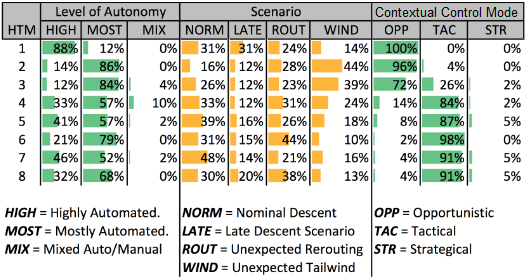
\includegraphics[width=4.5in]{figures/GALE,decisions,Opp}

\fig{all}a:  Exp \#1. Decisions found by GALE,  all contextual control modes enabled.

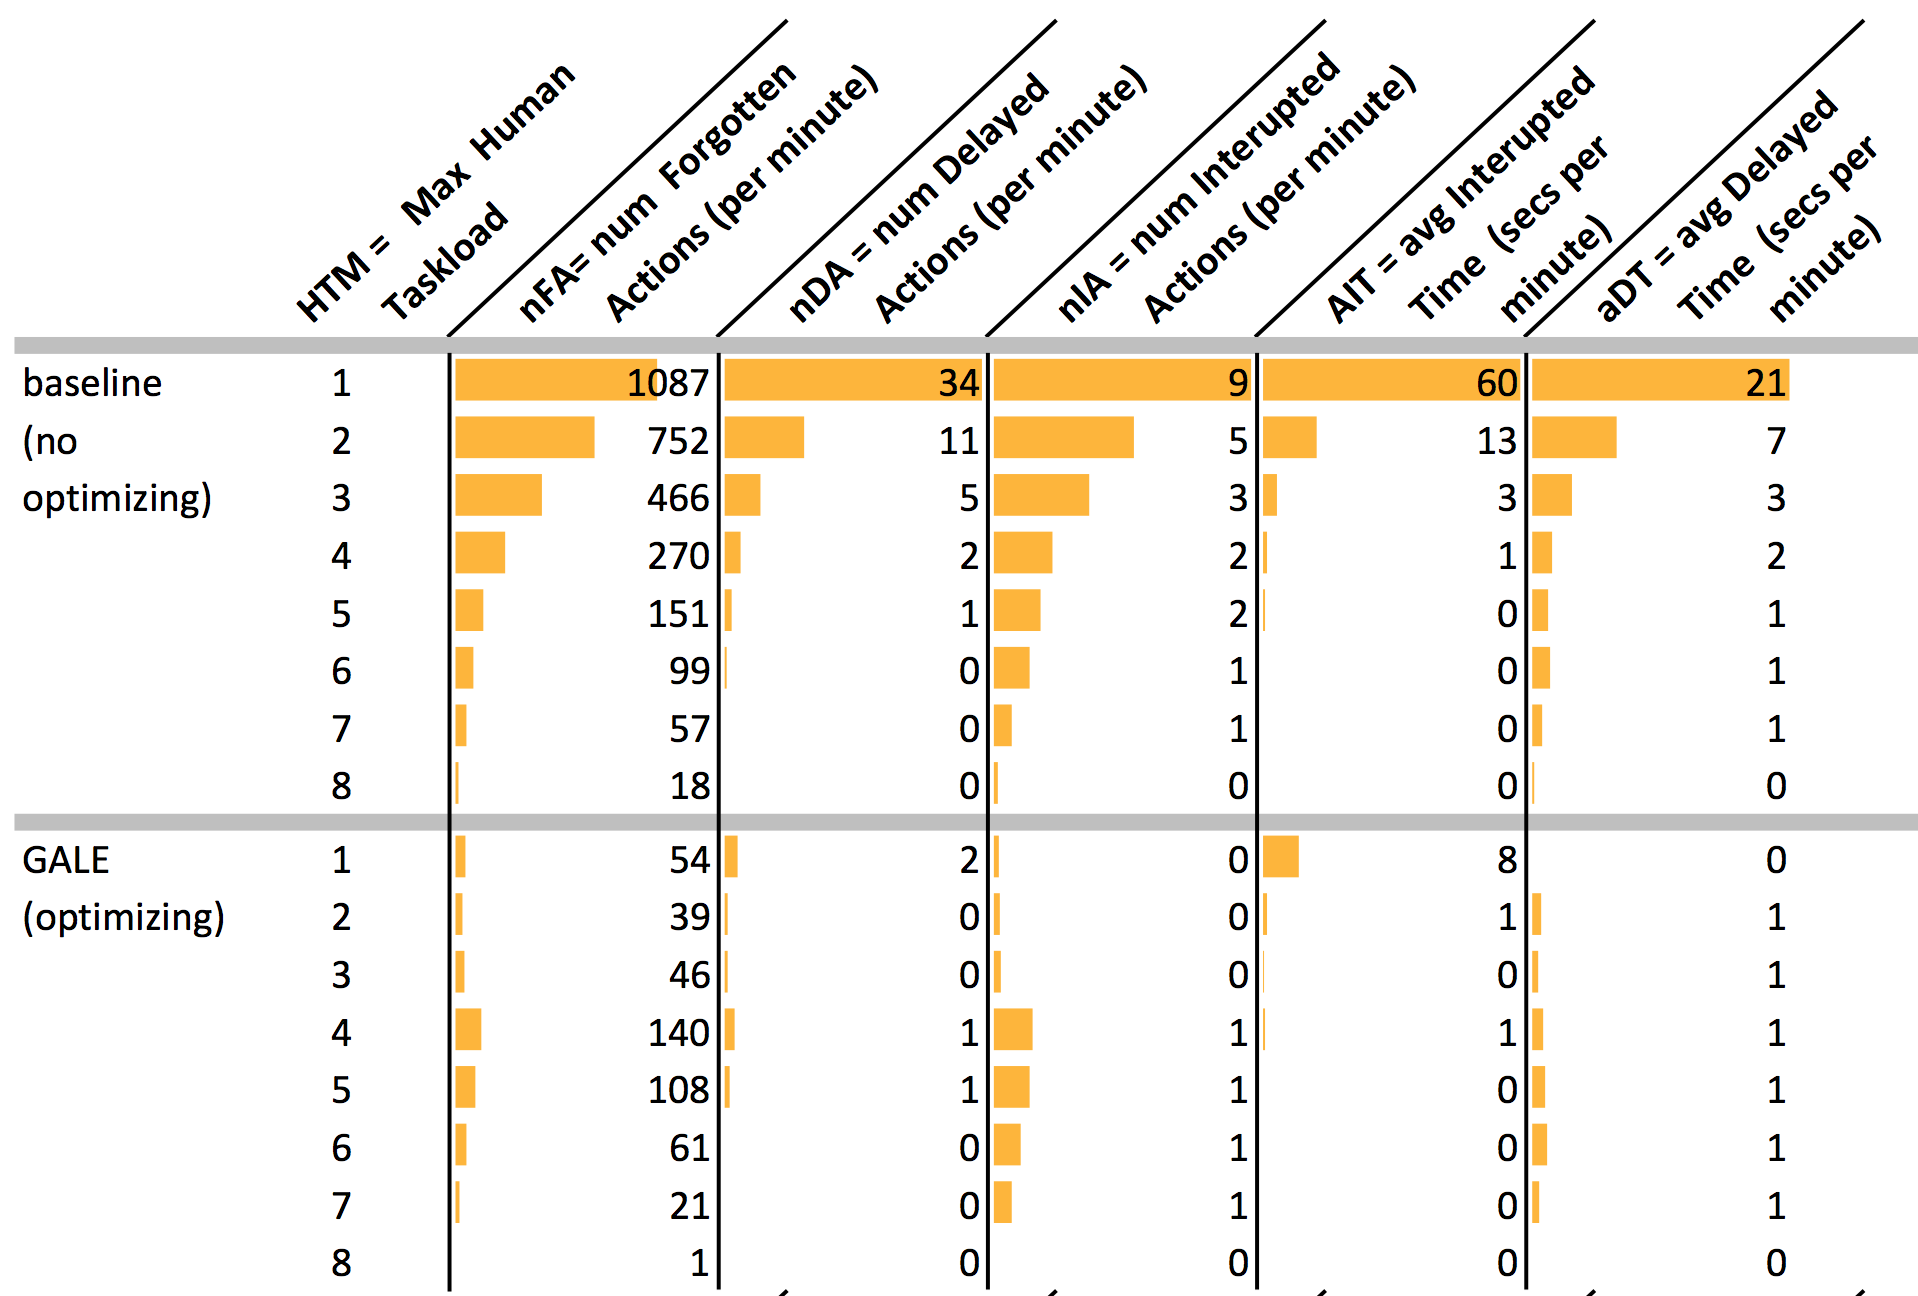
\includegraphics[width=5.25in]{figures/objectives,Opp}

\fig{all}b: Exp \#1.  Objectives obtained, all contextual control modes enabled.
\end{center}

\caption{Experiment \#1: All contextual control modes enabled. 
Forgotten, delayed, and interrupted actions are reported by the simulation at each 0.05s time step.  
E.g. a monitoring action can be `forgotten' 20 times each second.  }\label{fig:all}
\end{figure*}

\section{Results}
\subsection{Experiment \#1: Results}
\fig{all} and \fig{some} show the results of these two experiments.
As an aid to help visualization, bar graphs are added to each column (and the bar with the largest, smallest value shows the max,min values in the column).
In those figures, GALE's decisions are shown at top.
Beneath that, we show two sets of objective scores:
\bi
\item {\em The baseline runs} which are the average objective scores seen without using GALE (just from randomly selecting input decisions).
\item {\em The treated runs} which are the average final objective scores seen after 20 runs of GALE.
\ei
For the tables of objective results:
\bi
\item The controlled value (HTM, maximum human task load) is shown on the left hand side of the table.
\item The values in the other columns are all counts per simulated minute.
\ei
When reading these results, it is insightful to look for {\em saturation}, {\em trends}, {\em absences} and {\em cliffs}. 


\subsubsection{Saturation}

Values {\em saturate} when they are driven towards their theoretical maximum. 
In the case of the CDA objectives, any {\em Time} objective that occurs at 60 seconds per minute is {\em saturated}. 
Such saturation can be observed in the {\em avg Interrupted Time} and the {\em avg Delayed Time} values of 60 at  $\mathit{HTM}=1$ in \fig{all}b and \fig{some}b.

In terms of a pilot maintaining safe operations, saturation is highly undesirable. At saturation, a pilot is permanently interrupted for all tasks so everything gets delayed.  
Note that this saturation result satisfies  one of our {\em sanity checks} (that less HTM leads to more problems).

The good news is that saturation can be avoided. 
In \fig{all}b, we see that the simulated pilots following GALE's advice never
reach saturation at $\mathit{HTM}=1$.
GALE advises the simulated pilots to restrict themselves to only the most important tasks (in CDA's model, this means operating in {\em opportunistic} mode) and to allow the automation to handle all or most of the tasks that the automation can handle.
Note that this  means that our experiment satisfies  another {\em sanity check} (that GALE can learn mitigations to the low HTM problems).



\subsubsection{Trends}

{\em Trends} are  values that change  smoothly with changes to HTM. For example, the  {\em num Forgotten Acts} per minute is low in all results until HTM falls below four (after which time it can spike to alarmingly large values). 

With one exception, this trend holds for all objectives---which is to say that airplane safety is critically dependent on this HTM value.

The exceptions to this trend are the GALE results of \fig{all}b.  
In those rows, GALE could learn mitigations that compensate for pilots struggling to control. 
Those mitigations are shown in \fig{all}a. 
 

\subsubsection{Absence}

Several columns in \fig{all}a and \fig{some}a contain nearly all zero values. That is they are mostly {\em absent} from the recommendations made by GALE.

Sometimes, these absences are not informative.  
For example, in \fig{some}a, the absent values in {\em OPP} are the result of that experiment (this mode was disabled for that experiment).
But other absent columns are more interesting:
\bi
\item
A {\em MIX}ed level of autonomy was rarely useful, suggesting that the simulated pilots should very rarely program the computer to handle only some of the airplane instructions.
\item
Similarly, the {\em STR} strategic cognitive control mode was also rarely used.
From this result, we say that, in this model, pilots should avoid cycling through all of the available monitoring tasks while trying to anticipate future tasks.
\item Other absent columns can be seen in the scenarios GALE found it could handle. 
In \fig{some}b, GALE found that when opportunistic mode was disabled, it rarely could handle the {\em LATE} approach or high tail {\em WIND} situations.  
On the other hand, when opportunistic model was enabled, GALE's recommendations to the simulated pilot could handle all the {\em Scenario}s (see all the non-zero numbers in the {\em Scenario} columns of \fig{all}b).
\ei


\subsubsection{Cliffs}

{\em Cliffs} are values that change sharply between one HTM value and the next; there are two large cliffs in \fig{all}.

The first cliff relates to {\em Level of Autonomy}. 
At $\mathit{HTM}=1$, GALE nearly always selected for a {\em HIGH} level of autonomy. 
However, as soon as pilots can do or hold in memory two things at once (at $\mathit{HTM}>1$), that recommendation no longer holds.  
In fact, for all levels of $\mathit{HTM}>1$, GALE usually prefers for the pilot to process flight data and program the computer (i.e. to use the {\em MOST} approach).
\ADD{Another way to say this is that, when their attention is failing, our simulated human pilots should give more tasks to the machines.}
However, at any other time, it is better to guide, and not be guided by, the automatic systems.

The other cliff in these results is seen in the right-hand-side columns of \fig{all}a. 
In those results, it can be seen that for  $1 \le \mathit{HTM} \le 3$ the {\em OPP} (opportunistic) cognitive control mode is most often selected by GALE. 
However, above that point (for $\mathit{HTM}>3$), it is rarely selected.
This cliff is a large enough effect in  a critical range of the model to deserve special attention.
Accordingly, Experiment \#2 (discussed below) explores the the relative merits of opportunistic control versus other modes.

\subsection{Experiment \#2: Disabling Opportunistic Mode}
As shown in \fig{all}a, at low HTM levels of $\mathit{HTM}<4$, most of GALE's recommended actions use the opportunistic cognitive control mode (where pilots monitor and perform tasks related to only the most critical functions). 
To see if this was some quirk of the simulation, or an important effect, we repeated the above experiment with this opportunistic mode disabled.

The results are shown in \fig{some}.  
In those results, the following aspects are noteworthy:
\bi
\item Comparing the {\em baseline} and {\em GALE} distributions of  \fig{some}b, we see that the GALE treatment barely changes the baseline distributions. 
That is, if GALE cannot use the opportunistic control mode, then it cannot mitigate for low HTM values.
\item
Comparing the {\em Scenario} results in \fig{some}a to \fig{all}a, we see that when we cannot use opportunistic mode there are more absent columns in {\em LATE} and {\em WIND}.
That is, if GALE cannot use opportunistic control, then it cannot find another mitigation for late arrival or high wind conditions.
\ei
From these results, we say that opportunistic mode is an essential tool for combating the problems associated with low HTM in the CDA model.
 

\begin{figure*}
\begin{center}
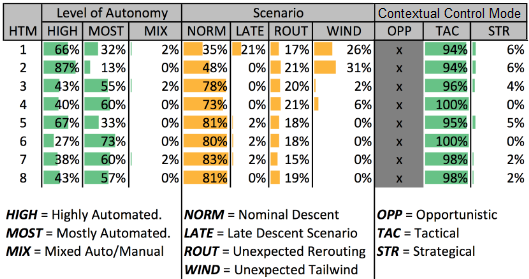
\includegraphics[width=4.5in]{figures/GALE,decisions,noOpp}

 \fig{some}a:  Exp \#2. Decisions found by GALE, opportunistic mode disabled.




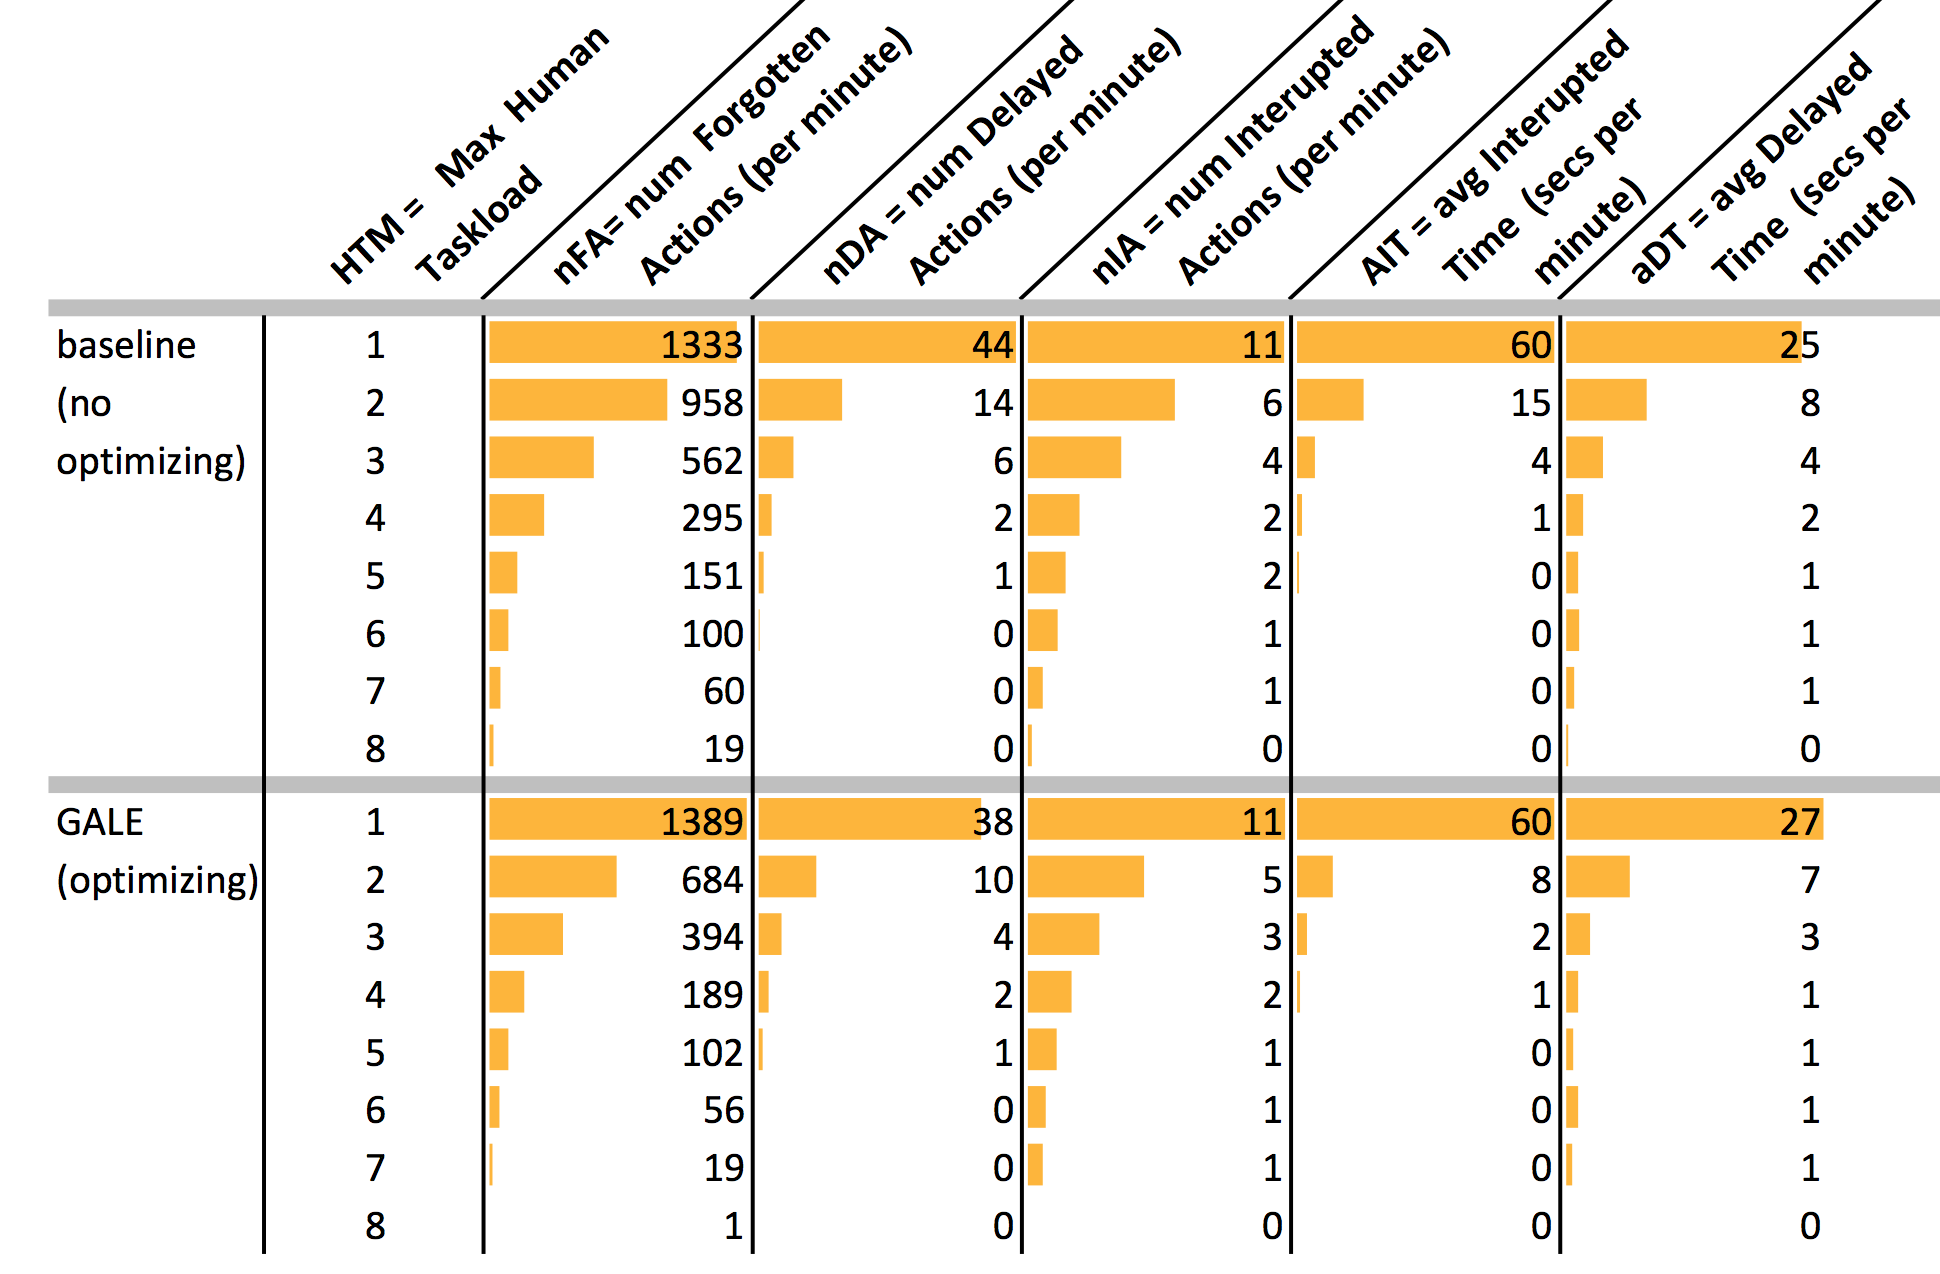
\includegraphics[width=5.25in]{figures/objectives,NoOpp}

\fig{some}b:  Exp \#2. Objectives obtained, opportunistic mode disabled.
\end{center}

\caption{Experiment \#2: Opportunistic mode disabled. 
See \fig{all} for a description of how the tasks are counted.}\label{fig:some}
\end{figure*}
%% \section{Analysis of Data}

%% standard params

%% runone: sanity check. effects of STM

%% solutions where we found best spread over varions scanarios

%% opp most important at low htm

%% The primary interest in this study was to explore the limitations of the pilots in the cockpit during approach to runway of a continuous descent profile (as in RQ1).  This section walks the reader through each experimental half (Including and Excluding Opportunistic), and each of the research questions are addressed as discussions become available for them.

%% \subsection{Half \#1: Including Opportunistic}

%% In~\fig{res1}, final and averaged objective scores (for each of the 20 repeats) are shown for the "Including Opportunistic CCM" half of experiments.  The objective scores should all be minimized for these experiments and orange bars are 'per-column'; the largest bar in each column represents the worst score for that column.  The bottom table represents the results after GALE was used to optimize those objective scores and the upper table represents the baseline objective scores without any optimization.  Those baselines were collected by running CDA a thousand times with randomized inputs (within respectively viable input ranges).

%% The message from~\fig{res1} is very clear: GALE was able to optimize those objective scores very impressively.  Even in the face of low HTM (which represents a workload that very highly exceeds pilot limitations), GALE was able to find inputs that could optimize the objectives.

%% The expectation prior to running GALE was met in the baselines: the objective scores were improved with higher HTM.  This addresses RQ1 and suggests that HTM directly has an effect on each of the objectives.  However, the GALE results confounded that expectation with a bell-shaped curve 'bump' occurring around HTM = 4.  This bump sparked an interest to further explore CDA by creating the "Excluding Opportunistic CCM" half of experiments, fueled by a hunch that the opportunistic CCM was the reason behind very strong GALE results across the objective scores.

%% Indeed, the story told by~\fig{res2} confirms that hunch.  That figure pulls out the inputs found by GALE to optimize the objective scores shown back in~\fig{res1}.  Each input is separated by input at the top level and then by possible value for that input at the second level.  Each row shows the percentage of inputs used for different levels of HTM.  A quick look at the Cognitive Control Mode (CCM) shows an identifiable trend where opportunistic (OPP) is chosen a vast majority of the time at low (1-3) levels of HTM, and then there is a paradigm shift at mid levels of HTM and higher (4-8).

%% %It is curious as to why results would be good at the extreme settings of low or high HTM, but not so well at medium HTM.  To explore that,~\fig{res2} shows the recommendations that GALE was making in its optimization of the objective scores.  For each set of columns (Level of Autonomy, Scenario and Cognitive Control Mode), each possible decision input is listed and the values shown in each row are the percentage of times that decision was recommended by GALE.  For instance, in the first row for HTM fixed to 1, the level of autonomy was set to "HIGH" 88\% of the time, and only 12\% of the time was it set to "MOST", and was never set to "MIX". 

%% This suggests that for RQ3, which explores the effect of changed CCM, that the lazier opportunistic mode is essential for optimizing objectives at lower HTM.  For higher HTM, opportunistic is less essential and tactical CCM is preferred instead.

%% Another identifiable trend from~\fig{res2} is in the level of autonomy input (function allocation, or FA).  For the lowest HTM (HTM = 1), the level of autonomy should be "HIGH" and other than that, it is clear that the "MOST" input value be used instead.  This makes sense, since at lower pilot HTM, the pilot is unable to keep up with the taskload pace, and there should be more automation to supplement that cognitive limitation.  This gives some insight into RQ2 and suggests that less autonomy for lower HTM could lead to larger backlogs of missed, delayed and forgotten tasks.

%% %Those decision recommendations of GALE show two very interesting trends.  Firstly, there is a clear trend in the level of autonomy for HTM settings of 1, where "HIGH" is very highly used, and otherwise, the "MOST" mode is used the most.  Secondly, for low HTM (1 to 3), the Cognitive Control Mode was generally preferred to be set to OPP (Opportunistic Mode).  Those two trends are outlined in bolder borders in~\fig{res2}.  To recap, the level of autonomy refers to the amount of work the computer does in the cockpit, and the cognitive control mode (CCM) refers to the monitoring behavior of the human pilot.  The OPP mode is a behavior mode where the human pilot is very relaxed and does not monitor flight activities very often, as opposed to TAC and STR which monitor flight activities increasingly more often.  At HTM settings of 4 or higher, the OPP mode was deferred and  TAC (Tactical) was preferred instead.

%% \subsection{Half \#2: Excluding Opportunistic}

%% Previously in the last subsection regarding the first half of experimentation, for RQ3, it was hypothesized that opportunistic CCM was essential to optimize the objectives.  To provide evidence of that, the opportunistic CCM was disabled and only tactical or strategic CCM was allowed for this second half of experiments.

%% The expectation is that without the opportunistic CCM, the objective scores cannot be optimized nearly as well as when opportunistic CCM is included.  In~\fig{res3}, which follows the same format as~\fig{res1}, that expectation is realized.  For low levels of HTM (1 to 3), GALE was unable to significantly improve objective scores from the baselines; the orange bars are basically unchanged in size (between baselines and GALE results).  For mid to high levels of HTM, the objective scores were already very low in the baselines and no optimization was needed - suggesting that random decision selection is satisfactory whenever there are little to no cognitive limits.

%% Going further, a look at the decisions recommended by GALE whenever OPP was disabled is shown in~\fig{res4}; there was no trend found for level of autonomy and the only decision GALE could tweak to find any performance increase at all was the scenario (but scenario is an uncontrollable decision in nature).  The CCM was locked in on tactical mode and strategical mode was hardly ever considered. 

\section{Discussion}

In principle, all the above conclusions could have been reached using an MOEA like NSGA-II. 
However, in practice, that would have been impractically slow. 
To understand why, we must review the systems-level tasks associated with conducting this kind of study.
Note that a discussion of these systems-level tasks rarely occurs in research publications. 
Researchers present only their final results and do not mention the work required before those results can be collected. 
In the case of this study, that work was quite extensive.  
{\em Commissioning} this CDA model took several months as one of us (Krall) worked inside the NASA firewalls to port the CDA model to the NASA servers. 
In that process, CDA was run many times to ``iron out the bugs''.  
Often it was necessary to trace through the evaluations to determine what was
going astray. 
During this period, we were grateful that GALE was only making $O(log(N))$ evaluations per generation since the $O(2N)$ evaluations used by standard optimizers would have led to an overwhelming amount of data.

Also note that after commissioning the model came {\em generating conclusions}.
This required 20 repeats of all models for baselines and with GALE, repeated for HTM set from one to eight, then repeated twice (for Experiment \#1 and \#2). 
With GALE, those runs took 83 hours and with NSGA-II, those runs would have taken much longer.
Based on some samples we made of NSGA-II performing parts of Experiment \#1, we estimate that if NSGA-II was used for the above experiments, then that would have taken 6 months.


As to the external validity of this work,
all the conclusions made here came from two tools: the CDA model and GALE. 
If these tools are somehow distorted or biased then our conclusions would be distorted or biased in the same manner.
That said,
there is enough  prior work on CDA and GALE  to make the case that it useful to study the CDA model with the GALE optimizer.
We note that these tools are the products of years of research and much analysis and testing ~\cite{Kim2011,Pritchett2011,Feigh2012,Kim2013,Pritchett2013,Pritchett2014, Feigh 2014,krall14aaai,krallphd,galepaper}. 
CDA is one of the largest and most studied models of pilot cognition currently available.  
Given the resources spent on its construction, it seems prudent and timely to learn what we can from that model.

%% Also, as to GALE, this algorithm uses a guided $log(N)$ heuristic to explore a space of $O(2N)$ possible comparisons (for details on this approach, see \tion{gale}). 
%% A pre-experimental concern with such an approach is that that this partial explanation of such a large space might miss some important details. Hence, this issue was extensively explored, using two dozen models, in Krall's thesis~\cite{krallphd}. 
%% In short, compared to $O(2N)$ algorithms such as NSGA-II~\cite{deb00afast}, GALE rarely performed worse and often performed better. 




\section{Conclusion}

A common, and naive, assumption made by researchers who have not conducted model-based experiments is this: once the model is built, then inference is easy.

We have shown in this paper that, for large and complex models, this naive assumption may not hold.
In fact, it is critically important to consider {\em how} that inference is conducted.
This paper endorses the use of modeling for complex studies, but it also addresses a few issues that must also be handled whenever learners are used in conjunction with models.  

Firstly, there is a need to develop and commission the model for integration
with the learner tools.  
This can be a time-intensive task and moreover, additional modifications can be cause for restarting the actual experimentation which follows thereafter.  

Secondly, the learners themselves are complex computational intelligence software tools which have been the subject of decades of research.  
The selection and deployment of just a single tool can become a complex decision
process.  
Moreover, high model runtimes can restrain the space of usable learning tools by a vast amount as much of the research on those learners has focused on optimizing very small models.  

In this paper, GALE was used because it can optimize very large models.  
This sort of enabling technology is made possible because GALE does not need to run the models as often as other learning tools (specifically, GALE performs $O(log(N))$ evaluations while standard methods explore a space of $O(2N)$ options).
GALE can quickly generate conclusions from complex models. 
For example, in the case study explored here we offer the following answers to the research questions posed in the introduction.




\subsection{RQ1: Safety and Low HTM}
We say that unsafe operation occurs if pilots cannot complete their assigned tasks.
For little to no cognitive limitations (HTM is 4 or higher), there is very little effect on taskload completion times.  
The reason for this is simple: if the pilot can perform all tasks as they come, then there should not be any backlog of delayed tasks.  
For lower levels of HTM, there were many delays and interruptions noted for our simulated pilots. 
Hence, we conclude that low HTM levels are especially dangerous within this model.

\subsection{RQ2: Impact of Automation}

For nearly all levels of HTM, it was sufficient to rely on a {\em MOST} level of autonomy where the pilot is in charge of processing input and programming the cockpit computers.
However, in extreme situations ($\mathit{HTM}=1$), that recommendation is not supported.  
For such very low levels of HTM, our simulated pilots should switch to {\em HIGH} levels of automation to ensure aircraft safety.
\begin{changed}
This recommendation intuitively makes sense if we assume that the automation works as the pilot intends.
Automation failures and automation surprise are beyond the scope of our study; we note that the creators of WMC have recently published a study with a version of their model tuned to study automation surprise~\cite{Gelman2014}.
\end{changed}

\subsection{RQ3: Pilot Monitoring Policies}

As to appropriate cognitive control modes for watching over an aircraft, for higher levels of HTM, it was sufficient to step up to the tactical control mode (which allows the pilot to monitor more of the aircraft flight procedures).
For lower levels of HTM, tactical flight operations proved to be too much for our
simulated pilot to handle and opportunistic control mode was essential to mitigate against low HTM.

\begin{changed}
More validation should be done before applying the recommendations we make here for the CDA model to the real-world safety problems that have inspired both CDA and this study.
However, our findings intuitively make sense.
In both the AirFrance and Asiana accidents that we used in our motivation, a key finding was that the pilots became distracted by off-nominal behavior, and {\em failed to monitor} the most important flight state information (e.g. airspeed, altitude and attitude).
When stressed, pilots are asked to do something very like the opportunistic mode as implemented within the CDA model---worry about the key monitoring and flight tasks first.
\end{changed}



%% Secondly, the results of applying GALE to the CDA
%% model for aircraft approaches are given in this
%% paper.  Those results can lead to large discussions,
%% but the general message is as follows: cognitive
%% limitations can be a serious detriment to taskload
%% completion times.  It is not a far stretch to
%% believe that high taskload completion times can lead
%% to decreased safety guarantees.  Moreover, a look
%% into the mitigations required to get around those
%% cognitive limitations shows that pilots rely on
%% automation within the aircraft whenever they cannot
%% handle the size of the taskload.  This point
%% combined with the most recent of aircraft accidents
%% raises an alarm because recent crashes have been the
%% result of over-dependence on autonomous agents when
%% those agents have been disabled or malfunctioning
%% during the approach.  Without the experience to land
%% the aircraft without the aid of the autonomous
%% agents, the pilot is faced directly against
%% cognitive limits and inexperience.

\section*{Acknowledgements}

The work was funded by NSF grant CCF:1017330 and the
Qatar/West Virginia University research grant NPRP
09-12-5-2-470.  This research was partially
conducted at NASA Ames Research Center. Reference
herein to any specific commercial product, process,
or service by trade name, trademark, manufacturer,
or otherwise, does not constitute or imply its
endorsement by the United States Government.

\bibliographystyle{IEEEtran}

\bibliography{references}
\newpage
\begin{IEEEbiography}[{
\includegraphics[width=1in,clip,keepaspectratio]{images/joe.png}} ]{Joseph Krall}
(Ph.D., WVU)
is a Postdoctoral Research Fellow funded by the National Science Foundation and is employed  at
LoadIQ, a high-tech start-up company in Reno, Nevada that researches and investigates cheaper energy solutions.
His research relates to the application of
intelligent machine learning and data mining algorithms to solve NP-Hard classification problems.
Further research interests lie with multi-objective evolutionary algorithms, 
search based software engineering, games studies, game development, artificial intelligence, and data mining.
\end{IEEEbiography}

\begin{IEEEbiography}[{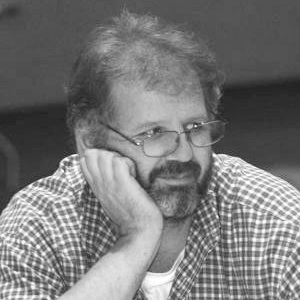
\includegraphics[width=1in,clip,keepaspectratio]{images/timm.jpg}}]{Tim Menzies} (Ph.D., UNSW)
is a Professor in CS at NcState and  the author of
over 200 referred publications. In terms of citations, he is one of the top 100 most
most cited
authors in  software engineering (out of 54,000+ researchers, see
http://goo.gl/vggy1). In his career, he has been a lead researcher on
projects for NSF, NIJ, DoD, NASA, as well as joint research work with
private companies. He teaches data mining and artificial intelligence
and programming languages. Prof. Menzies is the co-founder of the
PROMISE conference series (along with Jelber Sayyad) devoted to reproducible experiments in
software engineering: see http://promisedata.googlecode.com. He is an
associate editor of IEEE Transactions on Software Engineering. the Empirical Software Engineering Journal, and the
Automated Software Engineering Journal.  For more information, see his web site http://menzies.us
or his vita at http://goo.gl/8eNhY or his list of publications at
http://goo.gl/8KPKA .
\end{IEEEbiography}


\begin{IEEEbiography}[{
\includegraphics[width=1in,clip,keepaspectratio]{images/davies1_gs.jpg}}]{Misty Davies}
(Ph.D. Stanford),is a Computer Research Engineer at
  NASA Ames Research Center, working within the
  Robust Software Engineering Technical Area.  Her
  work focuses on predicting the behavior of
  complex, engineered systems early in design as a
  way to improve their safety, reliability,
  performance, and cost. Her approach combines
  nascent ideas within systems theory and within the
  mathematics of multi-scale physics modeling.
For more information, see her web site http://ti.arc.nasa.gov/profile/mdavies
or her  list of publications at
http://ti.arc.nasa.gov/profile/mdavies/papers.
\end{IEEEbiography}

\clearpage

\section*{Response to Reviewers}

\subsection*{Associate Editor's Comments}


Here are my suggestions

1.      Focus section 1 on GALE and its potential use in optimization of  models and do not focus on WMC or CDA at all. Explain that GALE could be used to analyze cognitive models that in general are very complex and thus could use model-based analysis frameworks such as GALE to make analysis more tractable.

{\em Yes. And following on from your suggestions, we moved much of section 4 into section1.}

2.      Delete section 2. I find it really is distracting. Pull the idea that there are too many analyses to run from section 2 into the new introduction but all the information about cockpit automation history and the 2 aviation examples are not necessary.

{\em Here, I'd like to push back just a little on your
editorial suggestions. 

Certainly, this section can
be extensively shortenned, and this draft does that. 

But I want
to point out that you work in this field and hence
you do not need a strong motivation to read this
paper.  

Please consider another kind of reader, one
who is only tangentially connected with this
work. That reader would need some "gentiling" in
order to read this article. For example, in terms of
supplying that motivation to read the paper, I
really like the phrase "a modern airplane is really
a computer with wings" and those graphics of
increasining fearsome cockpit complexity.

}

3.      Delete the current Section 3 (it should go into a case study)

{\em Agreed. We've wound an intro to CDA into the motivation section of 
the revised section 2.

}

4.  The current section 4 should really be section
2. However the material at its start about
model-based approaches should be moved to the new
introduction. Get rid of the discussion of what you
will explore later in the paper from section
2. Again no CDA, HTM, FA CCM and SC material should
go there. From 4.1 delete all of the material about
Kim’s thesis. The text in 4.1 could be very
short. The text up until “the problem here” could
just say simulations with many input parameters grow
in factorial space and there is a need for efficient
modeling techniques.

{\em Yes. Done.}

5.      I can’t really comments on Section 5 because this is your technology. However again take out all the CDA and WMC portions.

{\em Yes: and there is one para from there that works **much** better in the introduction anyway}.

6.      Now the new section 3 should be the methods for your case study and the new section 4 should be the results of your case study.

{\em Not quite, since I'm still trying to retain section2. But I think I've followed the spirit, if not the letter, of your suggestions}

7.      This new methods section should read like a methods section where you have apparatus, independent variables, dependent variables, data analysis and so on. In the way I read your paper, the WMC simulation was used to create data sets that you analyze using GALE. If I am incorrectly understanding this, of course then correct me. If I am right, you could explain WMC, the CDA model, the parameters it uses and the data set it creates in each run in an apparatus section. The dependent variables and independent variables sections would be those used by GALE. The data analysis part really  is the part where you describe how you ran GALE (pop size of 100 and so on).


{\em That ``Methods'' section is now divided as you said and  contains 
five sub-headings: (1) apparatus, (2) independent variables;
(3) depednent variables; (4) data analysis and (5) sanity checks.

}

8.      In your new results section you would have a subsection for exp 1 and one for exp 2

{\em Done}

9.      Section 6.6, 6.7 and Section 7 look like what should be in a discussion section

{\em Done.}

10.  Section 8 can also be deleted

{\em Ok}

I totally get it if you find this really annoying
but I hope you take these comments as a way to make
your paper relevant to the journal’s readers. I
think it could be shorter and focused on the story
you are trying to tell.

{\em No problem. Great to work with an editor that takes so much care and consideration!}


%% The present version of the manuscript is, I believe, close, but not quite at the point where it is ready to be published.  Reviewer 2 indicates that you have addressed all of his previous issues.  Reviewer 1 has a few very minor issues still to be addressed.  In contrast, Reviewer 3 identified many more issues to be addressed.  However, I believe that all of the issues, even the ones that Reviewer 3 can be handled with a very straightforward revision.  Most of the requested revisions involve clearer definitions, updates to information, and improved wording.  None require new analyses or reconceptualization of any section of the document.  Having noted that these revisions should be straightforward, let me also point out that they will improve the readability of your manuscript.

%% \begin{changed}
%% Thank you for these comments. As you say, the revisions for Reviewer1 and Reviewer2 are a simple matter.

%% As to Reviewer3, we really should have been clearer in the last draft on many points (see our remarks, below).

%% Note that all significant changes to this version are shown in blue.
%% \end{changed}


%% \subsection{Reviewer1 Comments}

%% Some more details about the case study implementation would be useful to facilitate the analysis of the results. 

%% Particularly, the impact on the recommended actions and GALE optimization results, between the different Cognitive Control Modes should be provided.

%% Some details about the comparison of GALE with standard optimization methods (NSGA-II) would be important to support the claimed research contribution.
%% \begin{changed}

%% We have added text throughout the paper on the case study implementation, and we have also included additional citation information for those who would like more details.

%% We have paid special attention to a clearer description of GALE's recommendations, particularly as they relate to the Contextual Control Modes.  (Per another reviewer's comment, we have more clearly recognized Hollnagel's contribution to the model by changing our terminology.  Cognitive Control Modes have become Contextual Control Modes throughout the paper.)

%% Thank you for the remark on the comparison of GALE to other optimization methods-- the previous version was weak on the connection of this approach to other MOEAs. We have added some notes on this topic on page 5 (please see the BLUE text there).
%% \end{changed}

%% \subsection{Reviewer 2 Comments}

%% Since this was a collection of papers that support the use of model-based analysis of human factors for safe aircraft approach the weakness that a reader may find is that there are parts in the later two papers that are repeated and/or glazed over. This is understandable with a compilation of three papers that were all designed initially to stand independent of each other. Without combining the entire collection of papers into a single work there is little that can be done to mitigate this redundancy regardless of its effect on the reader. 
%% \begin{changed}
%% Thank you for your understanding. As we said on page 1, this is not the paper that offers full details on GALE and we suspect that, like you, the interested reader will read on to the other papers.
%% \end{changed}


%% This title paper (first in the collection) did have a few grammar mistakes that are recommended to be resolved prior to the publishing of the piece.

%% \bi 
%% \item Paper 1 - Section 6.3.1: [Col 1|Line 34]: “where” should be “were”
%% \item Paper 1 - Section 6.3.2: [Col 1|Line 45]: “then” should be “where”
%% \ei
%% \begin{changed}
%% Typos fixed. Thank you for pointing those out.
%% \end{changed}

%% \subsection{Reviewer3 Comments}

%% I recommend the following:

%% 1)      Clearly define and operationalize your decision variables / inputs
%% HTM:  It is not clear what HTM is – presumably it stands for Human Task Load Maximum (but please confirm).  It is described as “an integer value ranging from 1 to 8, in which its value describes how many tasks can be handled at once before there are incurred delays, errors, or the possibility of the task being forgotten or lost”.    However, the number of pilots tasks can handle at once depends on the task and the resource modality.  For example, I can do two things at once if they require difference resources  (i.e. view a display and manually control aircraft), but I cannot do two tasks at once if they require the same resources (i.e. make two different verbal callouts at the same time).  How is this accounted for in the model?  I don’t think any human operator can do 8 tasks at once …. Maybe you should define what you mean by ‘task’ and ‘at once’.

%% \begin{changed}
%% HTM was defined both in Figure 2 as an acronym for this paper, and also as one of the decision variables (in bold) in the description of CDA in Section 3.  You are correct that it stands for maximum human task load.  We have expanded the definitions of the four decision variables, which will hopefully lead to less confusion for future readers.  

%% Per your recommendation, we have also made it more specific as to what we mean by 'task', and have provided the reference for the in-detail description (which takes many pages in the original reference). 
%% \end{changed}

%% Functional Allocation.  The distinction among the three categories of FA  (highly, mostly, and mixed) are unconventional (from the literature) and not clear. For example, in mixed-automation which tasks were ‘handled’ by the computer and how is that determined? It is not clear how Highly and Mostly are different.   I am confused by the wording ‘processes the instructions’ vs. ‘handle the task’.  Maybe some examples would help. How can the computer ‘process’ flight instructions in the highly condition, if they were not first programmed by the human.  And then, how is that different than mostly automated?  Not clear what is the difference between Mostly and Mixed.  What are examples of instructions that the computer handles in Mostly that the human handles in Mixed?

%% \begin{changed}
%% We have added text to make it clear what we mean by these function allocation levels, and also have added references for the interested reader.
%% \end{changed}

%% The definition of the CCMs are unconventional – I assume you are using Hollnagel’s Contextual Control Model as the basis for your work, despite that it is not referenced and you call it Cognitive Control Modes, not Contextual Control Modes.  As an example, you define ‘Tactical’ as “Cycling through most of the available tasks and double-checking some of the computer’s tasks”.  where as, Hollnagel defines it as follows:  “Tactical  is characteristic of situations where the person’s event horizon goes beyond the dominant needs of the present, but the possible actions considered are still very much related to the immediate extrapolations from the context.” (Hollnagel, 1993, pp. 170)” .  How do you reconcile the difference in definitions? How do you operationalize ‘most’ and ‘some’, how does the model decide with tasks to ‘cycle through’ and which to ‘double check’, and what is the difference between cycling and double-checking?

%% \begin{changed}
%% You are correct.  The implementers of WMC used Hollnagel's work as a basis for the model. We were working from a thesis that referred to these as cognitive control modes, but they are based on Hollnagel's Contextual Control Modes.  We have cleaned up the text to reflect this, and have also provided references to texts in which the exact implementation of these within WMC is described.
%% \end{changed}


%% Section 6.3.1, page 7.  …”Pilots made their own estimation on what where[sic] the most critical instruments to watch, and ignored all other.”  Since there were no actual pilots in this experiment, and it was a modeled-pilot was making the decisions – what criteria did the model use to decide what instruments to monitor?  For Example, Chris Wickens has a 4 parameter model called SEEV, which suggests pilots consider Salience, Expectancy, Effort, and Value – what did your model use?

%% \begin{changed}
%% You are correct that we should have been more specific -- the CDA model ranks the priorities of the monitoring tasks.  We have summarized the model assumptions and provided a reference.
%% \end{changed}

%% 2)      Clearly define your 5 Objectives
%% Modeling whether tasks are delayed, interrupted, or dropped, is a complex problem – with several different possible strategies  (first in-first out, priority, criticality, salience etc).  How do you operationalize ‘forgotten actions’.  Does your model have a memory component?  Do you model long-term, short-term memory?  Do you use linear or exponential decay curves?
%% How do you operationalize interrupted tasks.  Is there a prioritization scheme.  Do you use first in first out, last in first out, prioritize by importance,  criticality? There is no discussion as to how this is modeled.  And since this is a major part of the output, it is hard to make sense of the output.

%% \begin{changed}
%% We've expanded the objective description, briefly discussed the priority scheme and memory model, and added citations.  
%% \end{changed}

%% 3)      Some clarification needed in  Results
%% Figure 6,page 8.  I am not understanding Number of Forgotten Actions per minute.  How can an operator ‘forget’ 1087 actions per minutes? How can there be 1087 actions in any given minute to be forgotten?  Please define what you mean by ‘action’.


%% \begin{changed}
%% The same task can be 'forgotten' at each time step -- many times in one minute.  We've added a description to the captions of both Figure 6 and Figure 7.
%% \end{changed}

%% Section 6.4.2 (bottom of section).  “The good news is that saturation can be avoided.  In Figure 6b, if the simulated pilots following GALES’s advice, they never saturate at HTM=1.”  It is unclear what  GALE’s advice was – or how a pilots would follow it.  In other words, you claim to have a found a mitigation that would be useful for pilots – but what is it????

%% \begin{changed}
%% We claim to have found a mitigation that is useful for the simulated pilots, not real pilots.  We will leave it to others (or perhaps to future work) to validate and to improve the WMC CDA model.  At HTM1, in figure 6a, you see that GALE decided that the simulated pilots should fly with high levels of autonomy and in the opportunistic contextual control mode.  The Scenario, for this case, mattered less (although it looks to me like the tailwind was harder to fly).  We believe the interpretation of the figure 6a is obvious, and that the results are consistent with common sense.
%% \end{changed}

%% Section 6.4.3  “.. GALE could learn mitigations that compensate for pilots’ control struggles.  Those mitigations are shown in Figure 6a”

%% \begin{itemize}
%% \item How do we know which of those mitigations in 6a are having the effect ? 
%% \item How is Scenario a mitigation?
%% \item How is CCM a mitigation – you can’t program a human to behave in opp, tac, or str modes.
%% \end{itemize}
 
%% \begin{changed}
%% 1st item: Level of autonomy, scenario, and CCM are inputs to this simulation. You can see, in 6a, which decisions GALE chose.  In 6b, you can see the results of those decisions on the output.  
%% 2nd item: GALE suggests: if you can only hold one item in memory, avoid flying with a strong tailwind. GALE can suggest this because the Scenario is an input to the simulation.  The simulation is not reality.  Also note that, even in the simulation, the Scenario mattered relatively little to the simulation.  As one example, GALE chose the normal and the late scenarios equally often in its optimization for HTM=1.  We do plan on future work in which we fix the Scenario (you are correct that, naively, this should more closely represent reality), and identified that with the first sentence in Section 8.
%% 3rd item:  We respectfully disagree that you can't program a human.  We believe that this programming is called \em{training}.
%% \end{changed}


%% 4)      Carefully review your conclusions and tie your model results to practical, mitigations that can actually be implemented.

%% For example, on Page 10, top left “From these results, we say that opportunistic mode is an essential tool for combatting the problems associated with low HTM”.  How is OPP a “tool”?  You can’t hand it to a pilot and tell them to use it.  CCM is a result of the context / environment  (e.g. if pilots are not fatigued, well-trained,  carrying out a nominal descent in good weather, they can act opportunistically, yet when one more of these factors are applied, the pilot shifts to tactical or strategic modes).  In other words CCM is a RESULT of the factors you model (taskload, off-nominal events), it does not MITIGATE them.


%% \begin{changed}
%% We believe very strongly that tying our results given the simulation to recommendations that should be implemented in reality is overreaching. The simulation still needs more validation.  While the creators of the WMC framework are working very hard both to validate and to improve their models, as evidenced by their impressive recent results and publications, it is our understanding that there is no current computer model that is well-validated enough to be used to provide recommendations to real pilots.  Such models can only suggest experiments to be performed with pilots in-the-loop.

%% OPP is a mode that can be can be selected as an input to the simulation.  Our results showed that if the pilot had  a working memory of one, they should switch to an opportunistic control mode (within the simulation).  If the simulation has a direct correlation with reality, the analagous action would be to train the pilot to operate in this way:  let the computer handle most of the flying (high level of autonomy), and switch to opportunistic mode (just pay attention to a few key actions).  We believe such modes of operation can be trained. CCM and Autonomy level are definitely mitigations in the context of the simulation.  While we have just speculated for your benefit as to how they could also be mitigations in the context of reality, we emphasize our earlier point about the necessity of further validation.
%% \end{changed}

%% Concluding that low HTM levels are especially dangerous to aircraft is not particularly helpful. What have we learned from this that will  make aviation safer?  We shouldn’t hire pilots that can only handle 1 item at a time?  I think what we need to answer is: What do we know about the context that results in pilots not being able to handle more than 1 task at a time?


%% \begin{changed}
%% We agree that the question you posed is a very important research question to solve, and likely to be much more valuable from an aviation safety perspective than the one we address in our paper.  Your question is beyond the scope of this paper, and beyond the model's ability to capture (according to our understanding).
%% \end{changed}

%% Saying that “MIX is almost never a good approach” is over-reaching.  MIX as modeled was not good, but it was not clear how it was modeled.  Maybe the model had the computer do the wrong tasks?


%% \begin{changed}
%% Our results must be interpreted in the light of how each of these options were modeled in the simulation.  Again, we are not stating that these are good results for reality (yet).  In order to make recommendations about reality, we need an extra validation step.
%% \end{changed}

%% Page 8, bottom left.  Concluding “Pilots should avoid cycling through all of the available monitoring tasks while trying to anticipate future tasks”  Calls into question the validity of this study.   Do you seriously anticipate that being part of an airline’s training protocol: “Do not act strategically”.


%% \begin{changed}
%% This study is not (yet) about reality.  Note that, in future work, we plan to measure flight deviations and other safety-related output metrics.  Our results say, for this model, if you want to minimize forgotten and interrupted actions (and associated delays) then don't cycle through all of the tasks and anticipate future ones.  Once we have added other safety metrics, I expect the landscape of what you should do will become more complicated, even within the context of the model alone.  Personally, we think the fact that we automatically discovered that high levels of autonomy and an opportunistic mode of operation decrease the number of forgotten and delayed actions appeals to common sense and makes the study more likely to valid -- certainly in the context of the simulation and perhaps in the context of reality, as well.
%% \end{changed}

%% Figure 9, bottom left. I think it is a bit of a leap to conclude: “when cognitively limited pilots should trust their machines”.  The decision to trust a machine or not should be based on properties of the automation that make is trust-worthy (e.g. reliability, false alarm rate etc).  One should have no reason to trust automation more when they are cognitively limited than when they are not cognitively limited.


%% \begin{changed}
%% Our notes above on the scope of our effort (e.g. results apply only to this simulation, and only for the output metrics we listed) apply here as well. That being said, we have softened our language throughout the paper to make it clear that we are not overreaching our scope.
%% \end{changed}

%% 5)      Relate your model results and conclusions back to the two case-studies your presented in the intro.
%% It is not clear to me how your analysis of workload, cognitive control modes, or function allocation could either ‘explain’ or ‘predict’ either the Air France or Asiana accidents you cite as motivation in your introduction.  Can you tie these back into the discussion?  You attributed the Asiana accident to pilots mis-understanding the automation.  It is not clear that any of your variables – taskload, autonomy levels, cognitive control modes shed any light on whether a pilot misunderstands information.


%% \begin{changed}
%% You are correct that we should have more clearly tied our results back to our motivation.  We have done so.  You are also correct that none of our variables can predict whether a pilot misunderstands information.  We have made our scope clearer throughout the paper.
%% \end{changed}

%% And some odds and ends:
%% Please revisit your review of the Asiana Flight 214 crash that starts on page 2 and determine if it can be updated since more information is known now about that accident.


%% \begin{changed}
%% Thank you. We have done so.
%% \end{changed}

%% Page 6, Section 6.1 and 6.2.  You set up your study with a goal of understanding pilots’ “lack of attention” – this wording puts blame on the human operator which is not merited… By calling it ‘lack-of-attention, you seem to be saying “if only pilots could just pay more attention, aviation would be safer…”  Rather, in the examples you provide in section 6.1, the pilots’ attention is appropriately redirected to attend to an emergency situation or unexpected flight situation .


%% \begin{changed}
%% It is hard to argue that a pilot's attention (or lack thereof) has no impact on safety.  There are certainly many other attributes that affect safety, but these attributes were beyond our scope.  We have tried to be more clear about our scope. We would also like to argue that, in the examples we provide, we believe the pilots attention may be {\em inappropriately} redirected.  One possible interpretation of the Asiana 214 crash is that the pilots were so worried about unusual and yet second-order-importance tasks (e.g. training) that they failed to monitor the most important flight state variables (airspeed and altitude). 
%% \end{changed}

%% Section 4.1  You compare ‘model-based approaches’ to traditional case-studies.  It is not clear what you  mean by traditional case studies.   Do you mean pilot-in-the-loop studies?  What is it about traditional case-studies that is expensive, time-consuming and difficult to reproduce?


%% \begin{changed}
%% We have changed the wording in the section to make it more clear.
%% \end{changed}

\end{document}
XXX pragmatics
\subsection{Assembling the CDA Model}

The CDA model as used for the study required some integration with the search tools used in this paper and it was not ready-made for the task at hand.  The Work Models that Compute (WMC) framework had already implemented CDA but inputs and outputs had to first be selected to define the CDA model as a "problem instance" that the search tool can "solve".  This integration was performed by the first author of this paper during a summer internship with NASA Ames Research Center; WMC and the CDA model remains a Georgia Tech proprietary model accessible only via remote-access servers that connect to the machines located at NASA Ames.

CDA is just one "work" model contained within the Work Models that Compute (WMC) framework, with major contributors~\cite{Kim2011,Pritchett2011,Feigh2012,Kim2013,Pritchett2013}.  

Hence, CDA is a complex model that takes about 8 seconds to run.  That runtime was measured from a NASA Ames Linux server running on a 2.4gGHz Intel Core i7, with 8GB of memory.

Analysts at NASA have a lot of scenarios they would like to explore with CDA.  Given standard MOEAs like NSGA-II or SPEA2, that exploration would require 300 weeks to complete.  With GALE however, that time can be considerably shrunk, so the CDA model is an excellent candidate to demonstrate the true potential of such an active learner.




